\chapter{Visualización de imágenes 3D}
\label{chap:visualizaImagenes}
En éste trabajo estamos interesados en visualizar campos escalares discretizados. Un campo escalar es un mapeo $f:\mathbb{R}^3 \rightarrow \mathbb{R}$ donde $f$ típicamente representa el valor de una cantidad física en el espacio. En la actualidad muchos dispositivos, por ejemplo los tomógrafos, son capaces de producir muestreos de estos campos. Dada la naturaleza electrónica de los dispositivos con los que medimos el campo escalar, en realidad se tiene una aproximación de $f$ que se obtiene, en general, muestreando de manera uniforme el espacio tridimensional. 

%Sean $I, J, K \in \mathbb{Z}^+$. Para todo $\langle i, j, k \rangle \in \left[ 1, I \right] \times \left[ 1, J \right] \times \left[ 1, K \right]$ y para todo $d \in \mathbb{R}^+$, definimos un vóxel como:
Para representar un punto en $\mathbb{R}^n$, alternativamente $\mathbb{Z}^n$, usaremos la representación $\textbf{p} \in \mathbb{R}^n$, alternativamente $\textbf{k} \in \mathbb{Z}^n$, y su $n$-tupla $\textbf{p} = \{ p_1, p_2,\ldots, p_n \}$ donde $p_i \in \mathbb{R}$, alternativamente $\textbf{k} = \{ k_1, k_2,\ldots, k_n \}$ donde $k_i \in \mathbb{Z}$. Debido a que usamos recursos finitos para llevar a cabo la discretización de $f$ solo usaremos un subconjunto $\Gamma \subset \mathbb{Z}^3$ definido de la siguiente manera:

\begin{equation}
\Gamma = \left\lbrace \textbf{k} | A_i \leq k_i \leq B_i \text{ para } 1 \leq i \leq 3 \text{ con } A_i < B_i \text{ y } A_i, B_i \in \mathbb{Z} \right\rbrace 
 \label{ec:escena}.
\end{equation}

Dado un punto $\textbf{k} \in \Gamma$ y un numero real positivo $\Delta$, definimos un vóxel cúbico como 
\begin{equation}
   \text{Vox} (\textbf{k}) = \left\lbrace \textbf{x} \in \mathbb{R}^3 | \Delta \left(  k_i - \dfrac{1}{2} \right) \leq x_i < \Delta \left(  k_i + \dfrac{1}{2} \right)  , \text{ para } 1 \leq i \leq 3 \right\rbrace 
  \label{ec:voxel},
\end{equation}al número $\Delta$ comúnmente se le conoce como distancia de muestreo\cite{edgarReconstruction}. El termino vóxel proviene del ingles \emph{volume element} y por lo tanto pueden existir vóxeles no cúbicos. Al mismo tiempo un punto $\textbf{k} \in \mathbb{Z}^2$ tiene asociado un píxel, proveniente del ingles \emph{picture element}. Debido a que en éste trabajo no utilizamos teselaciones no cúbicas, usaremos el término vóxel para referirnos a los vóxeles de \eqref{ec:voxel}.

Al subconjunto $\Gamma$ de $\mathbb{R}^3$ para el cual esta definido $v$ se le llama \emph{escena}. De manera convencional a cada uno de los límites de las dimensiones del dominio de $v$ se le da un nombre. Típicamente al intervalo valido de $k_1$ se le conoce como el \emph{ancho} de la imagen, al intervalo de $k_2$ como la \emph{altura} de la imagen y al de $k_3$ como la \emph{profundidad} de la imagen.

Los vóxeles también pueden verse como la vecindad de Voronoi de un conjunto de puntos dispuestos como un arreglo rectangular que llena la escena\cite{Gabor:DigitalSpaces}, a este arreglo de puntos lo llamamos rejilla cúbica simple (\emph{sc}). Aunque de momento solo se hace uso de rejillas \emph{sc} estas no son las únicas formas de muestrear de manera uniforme el espacio, también existen otras rejillas como la \emph{face-centered cubic grid} (\emph{fcc}) o la \emph{body-centered cubic grid} (\emph{bcc}) que cubren el espacio de vóxeles con forma de rombo dodecaedros y de octaedros truncados respectivamente \cite{Gabor:DigitalSpaces}.

%Se hace la aclaración de que el término vóxel viene de \emph{volume element}, que es una generalización de su análogo de dos dimensiones \emph{píxel} de \emph{picture element}. A la teselación del espacio $\mathbb{R}^3$ en vóxeles como están definidos en la ecuación \eqref{ec:voxel} se le conoce como \emph{rejilla cúbica simple} (sc). A la distancia $d$ la llamamos \emph{distancia de muestreo}.

Dado un campo escalar $f$ y un intervalo de muestreo $\Delta$, definimos una digitalización como
\begin{equation}
  p_{\Delta}( \textbf{k} ) = \dfrac{1}{\Delta^3} \int \limits_{\text{Vox} ( \textbf{k} )} f(\textbf{x}) d\textbf{x}.
  \label{ec:digitalizacion}
\end{equation}

La digitalización definida en \eqref{ec:digitalizacion} da origen a una \emph{imagen digital} en 3D (o \emph{volumen}) que se define de la siguiente manera:
\begin{equation}
  v(\textbf{k}) =
  \begin{cases} 
      p_{\Delta}(\textbf{k}), & \text{ si } \textbf{k} \in \Gamma, \\
      0, & \text{ en otro caso.} \\                                
    \end{cases}
  \label{ec:imagen3D}
\end{equation}

Se espera que la imagen digital $v$ sea una buena aproximación del campo escalar $f$. Para que esto último sea posible deben pasar dos cosas. Primero que la distancia $|B_i - A_i|$ sean lo suficientemente grande como para abarcar todo el rango de interés del campo escalar $f$ y segundo, que la distancia $\Delta$ sea lo suficientemente pequeña para que los detalles importantes de la imagen no se pierdan debido a la digitalización expresada en \eqref{ec:digitalizacion} \cite{edgarReconstruction}. La principal limitante para lograr estas condiciones es que dependemos de la capacidad del dispositivo y de los algoritmos con los que se hace la digitalización. En este trabajo, sin embargo, se asumirá que no se tiene control del dispositivo del que se obtienen las imágenes, pero que se han obtenido ``buenas'' aproximaciones.

Al valor escalar $p_{\Delta}(\textbf{k})$ definido en \eqref{ec:digitalizacion} se le asocia una cantidad física que generalmente tiene que ver con la detección de la interacción de la materia que haya en el vóxel $\textbf{k}$ con cierta radiación. Aunque los tomógrafos proporcionan un valor $v(\textbf{k}) = \lambda \in \mathbb{R}$, algunas veces escalamos el rango de valores $r_i \leq \lambda \leq r_f$ a un cierto intervalo $[0, 2^i - 1]$ para algún entero positivo $i$.

En áreas como la medicina y la biología es común visualizar los volúmenes $v$ por planos o cortes generados al dejar fijo algún valor $k_i$ para alguna escena $\Gamma$. En medicina, si se trata de un volumen $v$ que aproxima un ser humano visto de pie, es común llamar a estos cortes como \emph{coronal} si divide al cuerpo humano en dos secciones adelante y atrás, \emph{sagital} si divide al cuerpo humano en secciones izquierda y derecha y \emph{axial} si lo divide en secciones arriba y abajo, ver Figura \ref{fig:cortesHB}. Sin embargo, este tipo de visualización tiene la enorme desventaja de perder la estructura tridimensional de la imagen, ver la Figura \ref{fig:imagenDigital}.

\begin{figure}[htp]
 \centering
  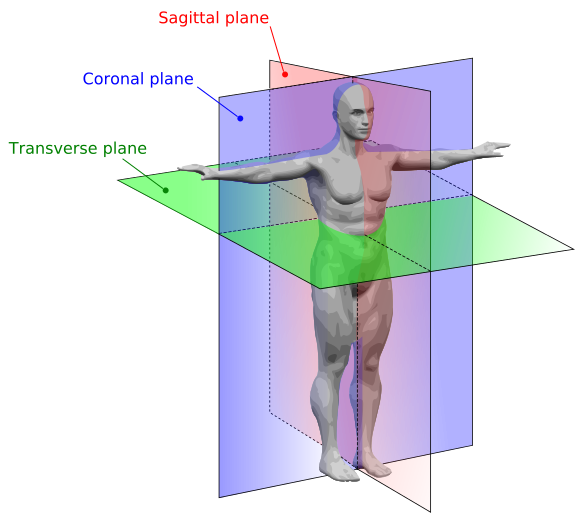
\includegraphics[scale=0.4]{img/cap01/HumanAnatomyPlanes}
  \caption[Cuerpo humano dividido en planos sagital, axial y coronal (La imagen fue tomada de \cite{wikiImagen})]{Cuerpo humano dividido en planos sagital, axial y coronal (La imagen fue tomada de \cite{wikiImagen}).}
  \label{fig:cortesHB}
\end{figure}

\begin{figure}[htp]
 \begin{center}
    \subfigure{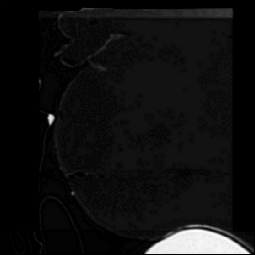
\includegraphics[scale=0.45]{img/cap01/01}}
    \subfigure{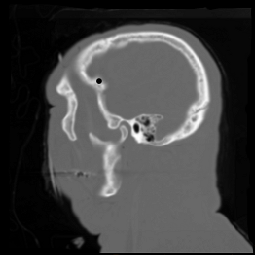
\includegraphics[scale=0.45]{img/cap01/02}} 
    \subfigure{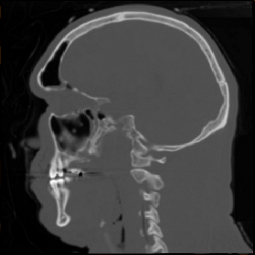
\includegraphics[scale=0.45]{img/cap01/03}} \\
    \subfigure{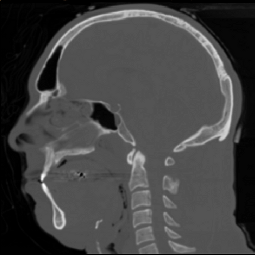
\includegraphics[scale=0.45]{img/cap01/04}}
    \subfigure{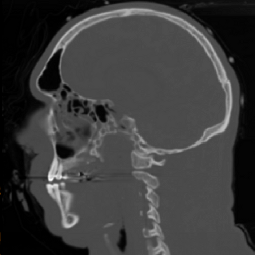
\includegraphics[scale=0.45]{img/cap01/05}} 
    \subfigure{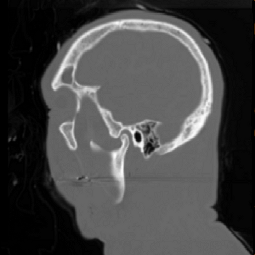
\includegraphics[scale=0.45]{img/cap01/06}}
  \end{center}
  \caption[Un volumen o imagen 3D visualizada por planos sagitales de una cabeza obtenida por medio de MRI (obtenida de \cite{visualHumanSite})]{Un volumen o imagen 3D visualizada por planos sagitales de una cabeza obtenida por medio de MRI (obtenida de \cite{visualHumanSite}).}
  \label{fig:imagenDigital}
\end{figure}

Por esta razón se han desarrollado formas de hacer una visualización completa de las imágenes que preserve la estructura 3D. Hay dos métodos generales de atacar este problema. La primera forma es conocida como visualización directa o \emph{volume rendering}. Este método fue originalmente propuesto por Drebin, Loren y Hanrahan en \cite{VolumeRendering} y hace uso de una técnica de GC conocida como \emph{alpha blending}. El método consiste en asociar a los vóxeles en la imagen $v$ una cierta función de transferencia y con ella calcular para cada vóxel $\textbf{k}$ un valor alfa (o de transparencia), de esta manera vóxeles con valores $p_{\Delta}( \textbf{k} )$ diferentes adquieren diferentes grados de opacidad. Esto permite ver todo el volumen directamente como una colección de objetos translúcidos. Un ejemplo se muestra en la Figura \ref{fig:volRender}.

\begin{figure}[htp]
 \centering
  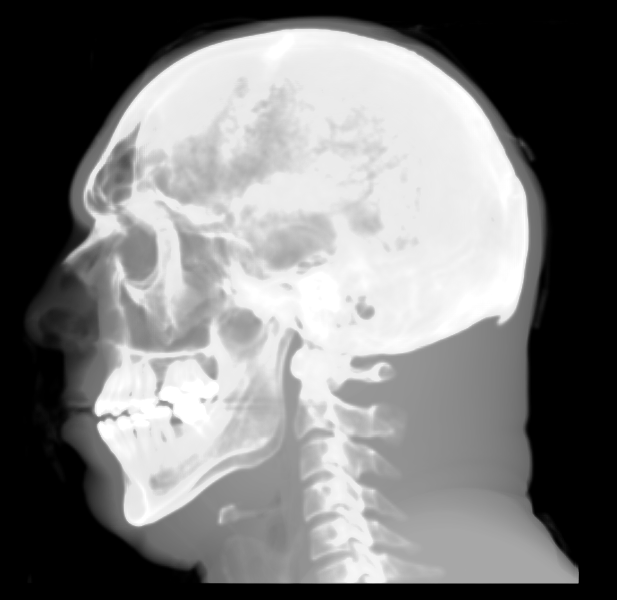
\includegraphics[scale=0.5]{img/cap01/volRender}
  \caption[El mismo conjunto de datos de la Figura \ref{fig:imagenDigital} visualizado por Volume Rendering]{El mismo conjunto de datos de la Figura \ref{fig:imagenDigital} visualizado por Volume Rendering. En esta imagen se usa el método de suma de intensidades como función de transferencia.}
  \label{fig:volRender}
\end{figure}

El otro método de visualización se llama \emph{visualización indirecta} o por superficies. Dado un campo escalar $f(\textbf{x})$, donde $f$ es una función escalar de $\mathbb{R}^3$, se define una superficie como sigue
\begin{equation}
S_{\tau} = \left\lbrace \textbf{x} \: | \: f(\textbf{x}) = \tau \right\rbrace 
 \label{ec:isosupeficie}.
\end{equation}
La superficie $S_{\tau}$ es llamada \emph{isosuperficie} o \emph{frontera} definida por $\tau$; el valor constante $\tau$ es llamado \emph{isovalor} o \emph{umbral}. Debido a que tenemos la aproximación $v$ de $f$, las técnicas por isosupeficie consisten en seleccionar un isovalor del conjunto de $p_{\Delta}(\textbf{k})$ (el rango de la imagen)  y rastrear la isosuperficie definida por ese valor. Esto resulta en una especie de envolvente o cascara discreta que forma una malla poligonal. Para poder definir la malla es necesario tener los vértices de cada polígono y la conectividad (saber que par de vértices forman cada arista). Esta malla se puede visualizar por métodos tradicionales de GC. En la Figura \ref{fig:visIsoSurface} se muestra el mismo volumen de las Figuras \ref{fig:imagenDigital} y \ref{fig:volRender} visualizado por cuatro isosuperficies correspondientes a diferentes isovalores en el rango $[0,255]$ y con el método de \emph{Marching Cubes}, explicado mas adelante.

  \begin{figure}[htp]
  \begin{center}
    \subfigure[$\tau = 61$]{\label{fig:mc61}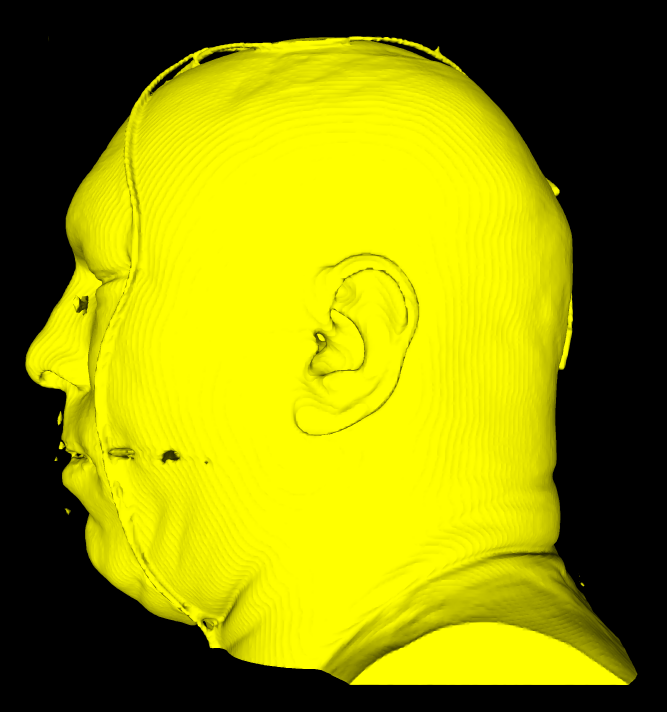
\includegraphics[scale=0.4]{img/cap01/mc61}}
    \subfigure[$\tau = 69$]{\label{fig:mc69}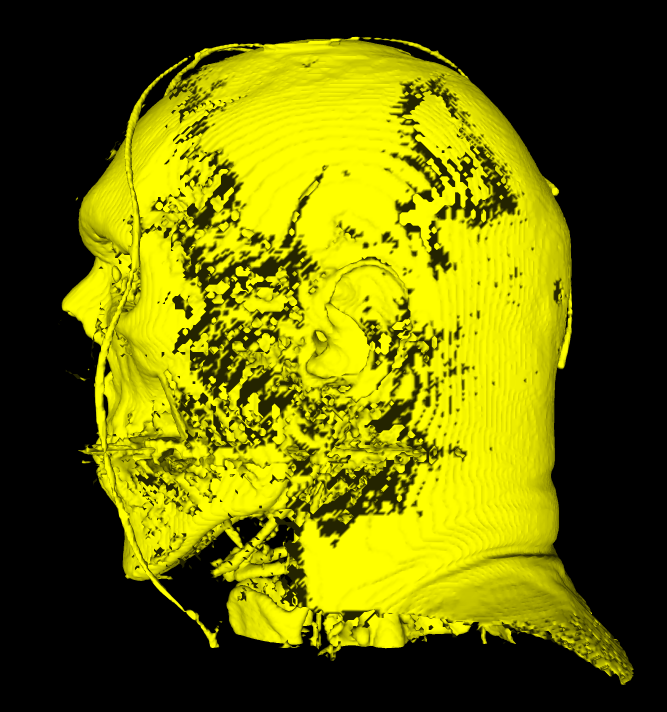
\includegraphics[scale=0.4]{img/cap01/mc69}} \\
    \subfigure[$\tau = 83$]{\label{fig:mc83}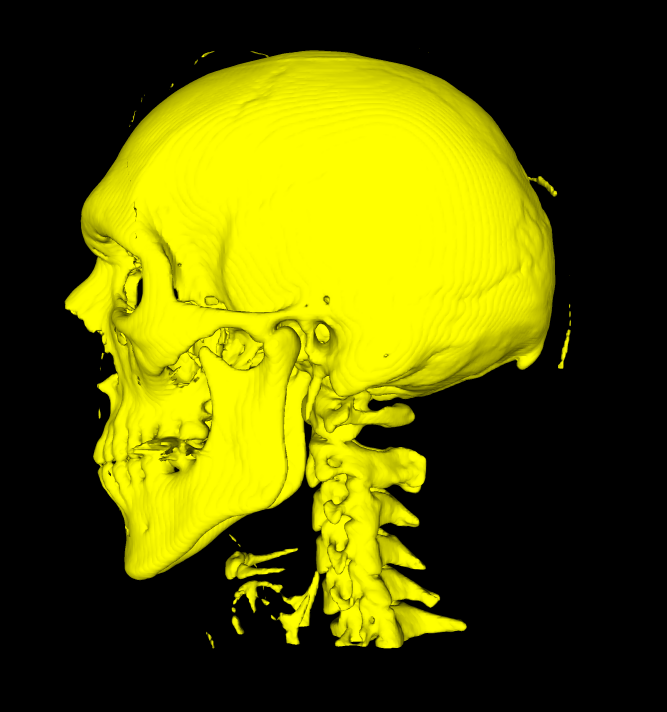
\includegraphics[scale=0.4]{img/cap01/mc83}}
    \subfigure[$\tau = 123$]{\label{fig:mc123}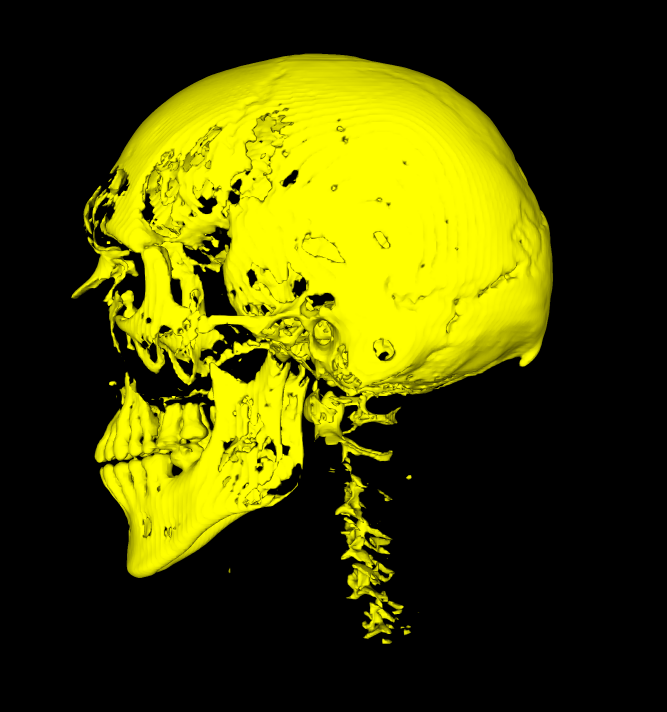
\includegraphics[scale=0.4]{img/cap01/mc123}}
  \end{center}
  \caption[Visualización por superficies de la imagen 3D de la Figura \ref{fig:imagenDigital} con cuatro isovalores distintos]{Visualización por superficies de la imagen 3D de la Figura \ref{fig:imagenDigital} con cuatro isovalores dentro del rango $[0,255]$ producida con el método de \emph{Marching Cubes}.}
  \label{fig:visIsoSurface}
  \end{figure}

Hay varias razones por las que la visualización por superficies es más usada. Por ejemplo la rapidez del cómputo y el hecho de que tanto el hardware como el software que usamos esta optimizado para visualizar estas superficies. Sin embargo, la mas importante es que los humanos estamos acostumbrados a ver las cosas de esa manera, generalmente solo percibimos la capa exterior de la mayoría de los objetos.
%El Algoritmo de Artzy tiene bastantes propiedades deseables ausentes en MC. Sin embargo, dado que éste último es el estándar contra el cual compararemos los resultados del trabajo es conveniente tener claro como funcionan ambos algoritmos.
\section{Generación de mallas}
\label{sec:generarMallas}
Hay varios algoritmos que pueden rastrear la frontera y construir la malla que la aproxima. El algoritmo de \emph{Marching Triangles}, propuesto por Hilton,  Stoddart, Illingworthy y Windeatt en \cite{marchingTriangles}, produce una malla a partir de una nube de puntos. En este algoritmo se empieza con un triangulo y se empiezan a añadir vértices que forman triángulos con las aristas que ya pertenecen a la malla, cuidando de cumplir que la triangulación que forma la malla sea siempre una triangulación de Delaunay. Este método tiene la enorme ventaja de producir mallas estables y de buena calidad. La desventaja de este algoritmo es que la malla resultante no suele adaptarse bien a las secciones de la superficie donde hay muchos detalles finos. En \cite{regionGrowingExtraction} se propone una mejora, capaz de producir mallas adaptables y además es capaz de encontrar los diferentes componentes conexos del volumen.

Otro algoritmo que fue propuesto por Keppel \cite{contoursKeppel} reconstruye la superficie a través de secciones transversales del volumen. En un primer paso en cada una de las secciones transversales extraen un contorno por medio de algún algoritmo de detección de bordes. En un segundo paso los contornos de secciones adyacentes se empiezan a unir formando polígonos. El paso crucial de este algoritmo es conectar de manera correcta los diferentes contornos. Sin embargo, debido a que los contornos que deseamos reconstruir en medicina son muy complejos no se logra hacer la conexión de manera aceptable. Por esto último se han escrito algunas mejoras (ver por ejemplo \cite{improvementCoutours}), pero debido a que la mayoría se basan en heurísticas estos métodos son poco usados en la actualidad \cite{focOnSciVis}. 

En éste trabajo estamos interesados en dos métodos: el método de \emph{Marching Cubes} (MC)\cite{MarchingCubes} que es el estándar mas usado actualmente y el Algoritmo de Artzy\cite{artzyCorto}.

\subsection{Adyacencias y caminos}

Antes de explicar como funcionan estos algoritmos necesitamos definir los conceptos de adyacencia y camino entre vóxeles

El concepto de \emph{adyacencia} entre dos vóxeles es una relación binaria simétrica sobre $\mathbb{Z}^3$. Se dice que dos vóxeles son vecinos cuando son adyacentes. Existen varias adyacencias, aquí solo vamos a utilizar dos de las más comunes.

Se dice que dos vóxeles $\textbf{c}$ y $\textbf{d}$ en la rejilla \emph{sc} son \emph{adyacentes cara a cara} o $\omega$-adyacentes, si difieren en sólo una de sus coordenadas, ver Figura \ref{fig:omegaAdyacencia}. Es decir:
\begin{equation}
(\textbf{c}, \textbf{d}) \in \omega \leftrightarrow |\textbf{c} - \textbf{d} | = 1 
\label{ec:adja6},
\end{equation} en donde $|\textbf{p}|$ denota la norma euclideana del vector $\textbf{p}$. Un vóxel en la rejilla puede ser adyacente bajo $\omega$ con otros seis vóxeles de la rejilla, es por eso que a esta adyacencia se le conoce también como la $6$-vecindad del vóxel, ver la Figura \ref{fig:vec6vecindad}.

%Otra posible adyacencia es la llamada \emph{adyacencia vértice a vértice} ó $\alpha$-adyacencia. Aquí se dice que dos vóxeles son adyacentes si comparten una cara, si comparten una arista, o bien si comparten un vértice. Ver Figura \ref{fig:alphaAdyacencia}. Se puede definir como:

%\begin{equation}
%(\textbf{c}, \textbf{d}) \in \alpha \leftrightarrow \left(  \textbf{c} \neq \textbf{d} \text{ y } |c_1 - d_1|, |c_2 - d_2|, |c_3 - d_3| \leq 1 \right)
%\label{ec:adja26}
%\end{equation}

%En esta adyacencia cada vóxel tiene 26 vecinos, por lo que también se le llama la 26-vecindad, se puede ver en la Figura \ref{fig:vec26vecindad}.

%Finalmente hay una tercera adyacencia llamada \emph{adyacencia arista a arista} o $\delta$-adyacencia. En ésta adyacencia los vóxeles son vecinos si comparten una cara o comparten una arista. Ver Figura \ref{fig:deltaAdyacencia}

Hay otra adyacencia llamada \emph{adyacencia arista a arista} o $\delta$-adyacencia. En ésta adyacencia los vóxeles son vecinos si comparten una cara o comparten una arista, ver Figura \ref{fig:deltaAdyacencia}. Esta adyacencia se define de la siguiente manera:
\begin{equation}
(\textbf{c}, \textbf{d}) \in \delta \leftrightarrow 1 \leq |\textbf{c} - \textbf{d}| \leq \sqrt{2}.
\label{ec:adja18}
\end{equation}

Esta adyacencia también se le llama la 18-vecindad porque el vóxel tiene 18 vecinos, ver Figura \ref{fig:vec18vecindad}. Se hace énfasis en que estas adyacencias son inclusivas. La $\delta$-adyacencia incluye a la $\omega$-adyacencia.%y la $\alpha$-adyacencia incluye a las otras dos.

Un $\pi$-camino de $\textbf{c}$ a $\textbf{d}$ se define como la secuencia de vóxeles $\langle \textbf{c}^0, \textbf{c}^1, \ldots, \textbf{c}^n \rangle$ tales que $\textbf{c}^0 = \textbf{c}$, $\textbf{c}^n = \textbf{d}$ y para todo $1 \leq i \leq n$ $\textbf{c}^{k-1}$ es $\pi$-adyacente a $\textbf{c}_{k}$. Un conjunto $A$ de vóxeles es $\pi$-conexo si entre cada par de vóxeles de $A$ hay un $\pi$-camino. Por lo tanto se pueden tener elementos $\omega$-conexos a través de un $\omega$-caminos y similarmente para la $\delta$-adyacencia.

\begin{figure}[htp]
 \begin{center}
   \subfigure[Vóxeles $\omega$ y $\delta$ adyacentes]{\label{fig:omegaAdyacencia}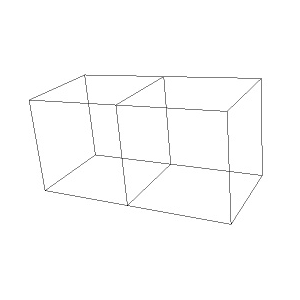
\includegraphics[scale=0.65]{img/cap01/omega}}
   \subfigure[Vóxeles $\omega$ adyacentes.]{\label{fig:deltaAdyacencia}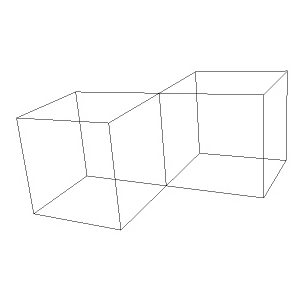
\includegraphics[scale=0.65]{img/cap01/delta}}
    %\subfigure[Voxeles $\omega$, $\alpha$ y $\delta$ adyacentes.]{\label{fig:alphaAdyacencia}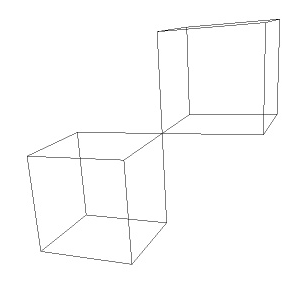
\includegraphics[scale=0.65]{img/cap01/alpha}} \\
  \end{center}
  \caption[Dos tipos de adyacencias típicas para vóxeles cúbicos]{Dos tipos de adyacencias típicas para vóxeles cúbicos.}
  \label{fig:adyacencias}
  \end{figure}

  \begin{figure}[htp]
  \begin{center}
    \subfigure[6-vecindad]{\label{fig:vec6vecindad}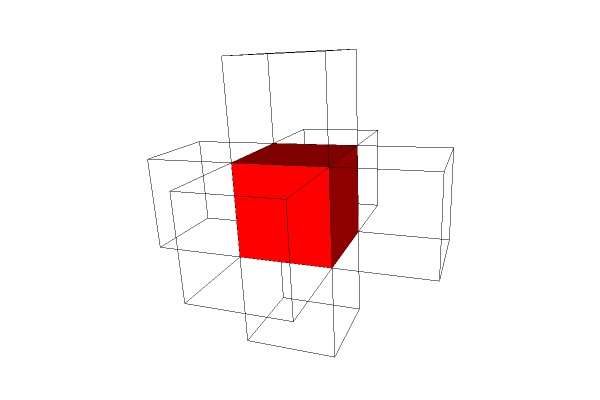
\includegraphics[scale=0.36]{img/cap01/vecindad6}}
    \subfigure[18-vecindad]{\label{fig:vec18vecindad}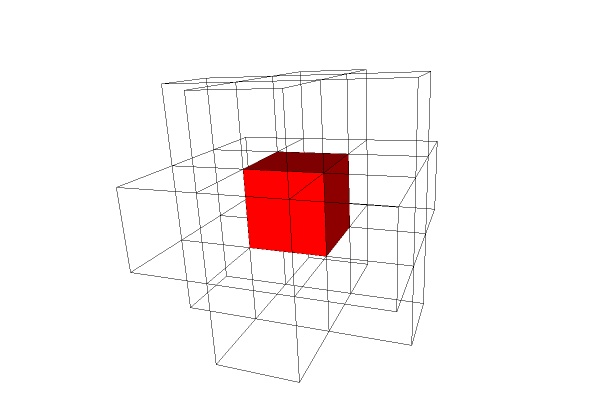
\includegraphics[scale=0.36]{img/cap01/vecindad18}}
    %\subfigure[26-vecindad]{\label{fig:vec26vecindad}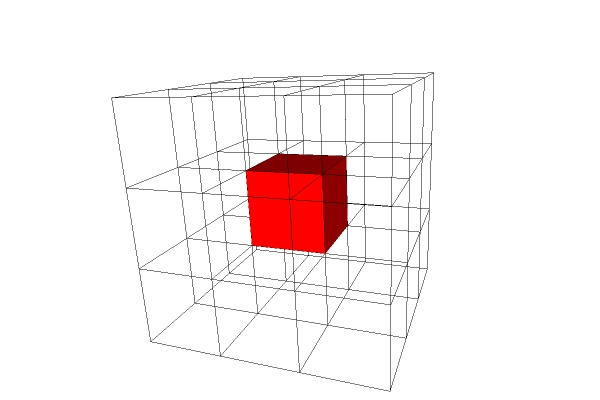
\includegraphics[scale=0.36]{img/cap01/vecindad26}} \\
  \end{center}
  \caption[Vecindades de un vóxel cúbico simple]{Diferentes vecindades de un vóxel cubico simple.}
  \label{fig:vecindades}
  \end{figure}


\subsection{El algoritmo de \textit{Marching Cubes} de Lorensen y Cline}
Este algoritmo fue propuesto inicialmente por Lorensen y Cline en \cite{MarchingCubes}. Al ser tan popular se ha escrito bastante acerca de sus propiedades, de sus puntos débiles y de sus posibles mejoras. Un resumen de todos estos trabajos puede verse en \cite{mcResumen}.

La entrada del algoritmo es un volumen $v$ junto con un umbral $\tau$. La salida es un conjunto de triángulos $\mathcal{M}_{\tau}$ que aproxima la superficie $S_{\tau}$ de \eqref{ec:isosupeficie}. El algoritmo consiste en hacer recorrer un cubo por el volumen, en cada parada se van generando los triángulos que forman $\mathcal{M}_{\tau}$, de ahí su nombre.

El algoritmo utiliza un cubo formado por los centros de ocho vóxeles contiguos de tal forma que para cada vóxel $\textbf{k} \in \Gamma$, el cubo tiene por vértices los centros de vóxeles $C(\textbf{k}) = \{ \textbf{k}^i | k^i \in \mathbb{Z} \text{, } \textbf{k}^1 = \textbf{k} \text{ y } 1 \leq i \leq 8 \}$ en donde: $\textbf{k}^{2} = (k_{1}^{1} + 1, k_{2}^{1}, k_{3}^{1})$, $\textbf{k}^{3} = (k_{1}^{1}, k_{2}^{1} - 1, k_{3}^{1})$, $\textbf{k}^{4} = (k_{1}^{1} + 1, k_{2}^{1} - 1, k_{3}^{1})$, $\textbf{k}^{5} = (k_{1}^{1}, k_{2}^{1}, k_{3}^{1} + 1)$, $\textbf{k}^{6} = (k_{1}^{1} + 1, k_{2}^{1}, k_{3}^{1} + 1)$, $\textbf{k}^{7} = (k_{1}^{1}, k_{2}^{1} - 1, k_{3}^{1} + 1)$ y $\textbf{k}^{8} = (k_{1}^{1} + 1, k_{2}^{1} - 1, k_{3}^{1} + 1)$, ver la Figura \ref{fig:barridoCubo}. 

Para cada voxel $\textbf{k} \in \Gamma$ se revisan los los valores de cada $\textbf{a} \in C(\textbf{k})$ que conforman el cubo, si el valor del vóxel $v(\textbf{a})$ es mayor o igual que el isovalor $\tau$, marca al vóxel como \emph{interior}, si el valor $v(\textbf{a})$ es menor que el isovalor lo marca como \emph{exterior}. Como en cada parada el cubo toca ocho vóxeles y cada uno de puede ser dentro o fuera, hay $2^8$ posibles casos. Si todos los vóxeles son interiores, el cubo esta dentro de la superficie y por lo tanto no hay nada que hacer. Si el valor de todos los vóxeles es exterior, el cubo está fuera de la superficie y tampoco hay que hacer.

\begin{figure}[htp]
 \centering
  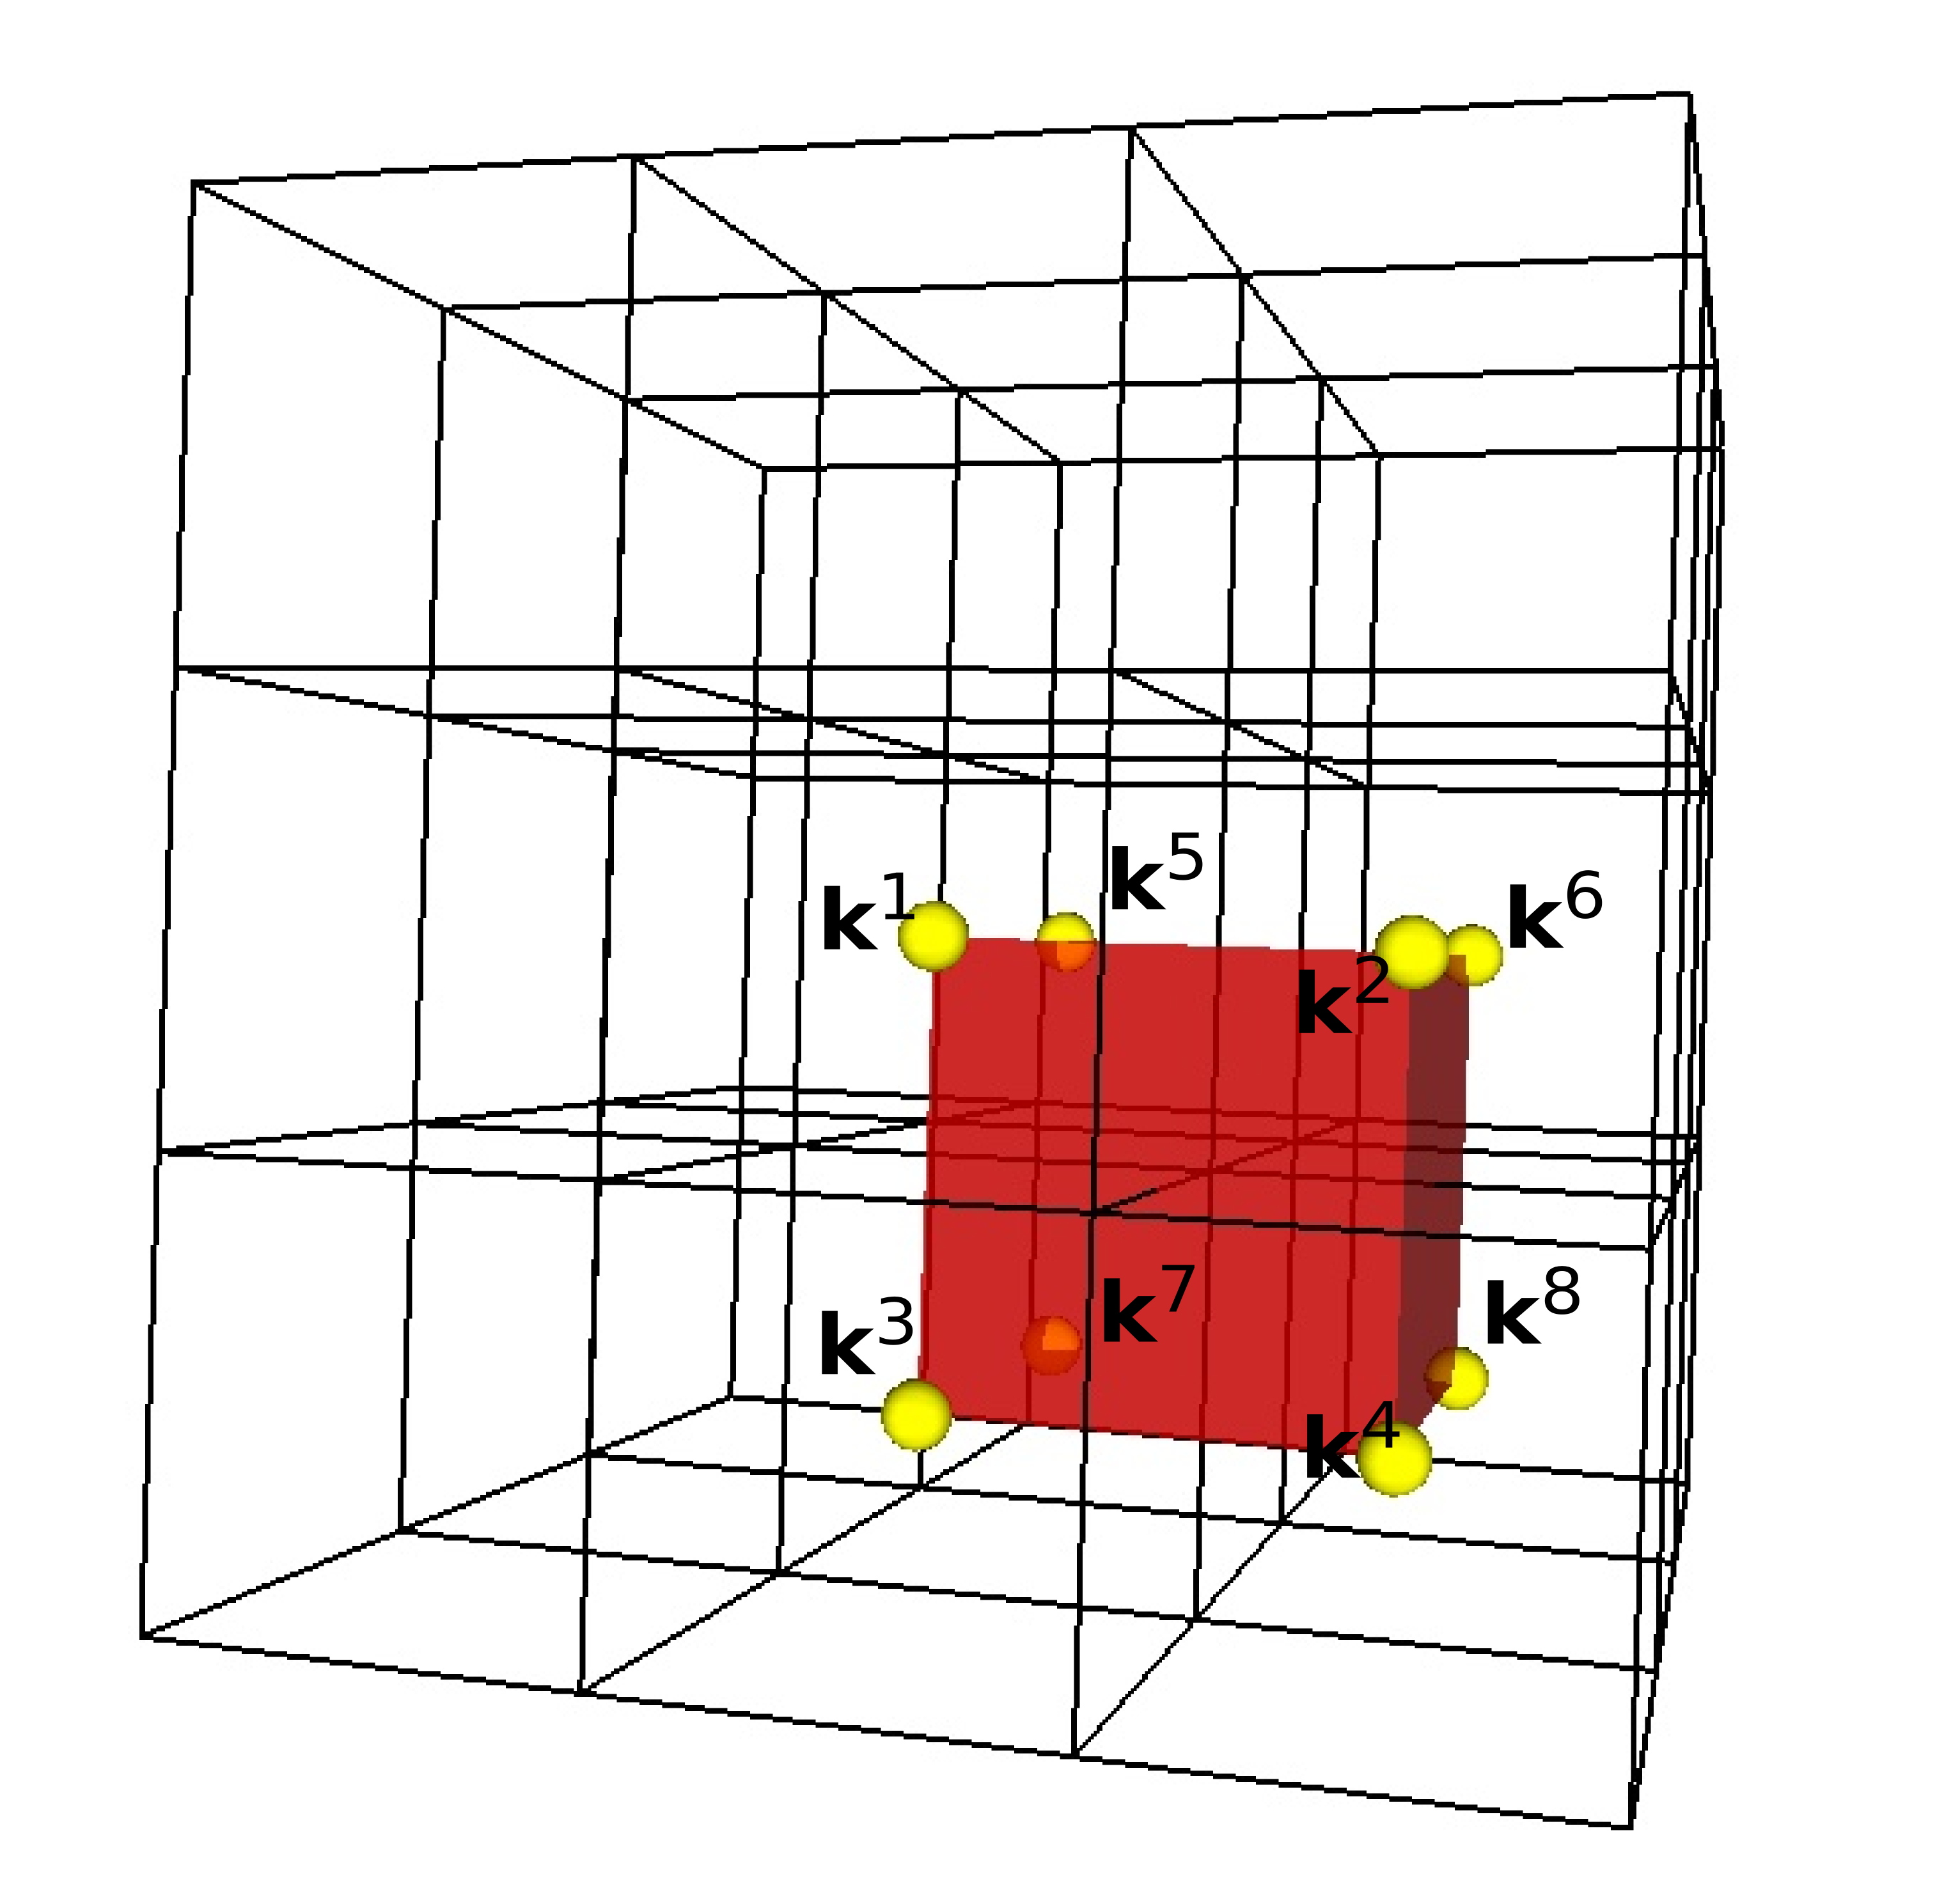
\includegraphics[scale=0.5]{img/cap01/mcCube}
  \caption[El algoritmo de MC utiliza un cubo formado con los centros de ocho vóxeles contiguos para recorrer el volumen]{El algoritmo de MC utiliza un cubo (ilustrado en rojo) formado por los centros de ocho vóxeles contiguos ilustrados por las esferas $\textbf{k}^{i}$ con $1 \leq i \leq 8$. Este cubo se va recorriendo a lo largo de todo el volumen $v$.}
  \label{fig:barridoCubo}
\end{figure}

Los casos interesantes son cuando hay tanto vóxeles externos como vóxeles internos, porque eso significa que estamos en un cruce de la isosuperficie. Cuando estamos en uno de estos casos hay que generar triángulos que aproximen la superficie. En el algoritmo original, la configuración de los vértices de los triángulos a generar en cada caso se guardan en una tabla que es construida manualmente.

El MC estándar considera que algunos casos son equivalentes de acuerdo a rotaciones y complementos. Un caso es complemento de otro si todos los vóxeles del primero tienen el marcado contrario en el segundo. Un caso es una rotación de otro si hay un conjunto de rotaciones que transforman al primer caso en el segundo. Por lo que se pueden clasificar las 256 configuraciones posibles en solo 15 casos. El la Figura \ref{fig:mcCasos} se ven todos los casos a los que se reducen las configuraciones una vez que se explotan los complementos y las rotaciones.

\begin{figure}[htp]
 \centering
  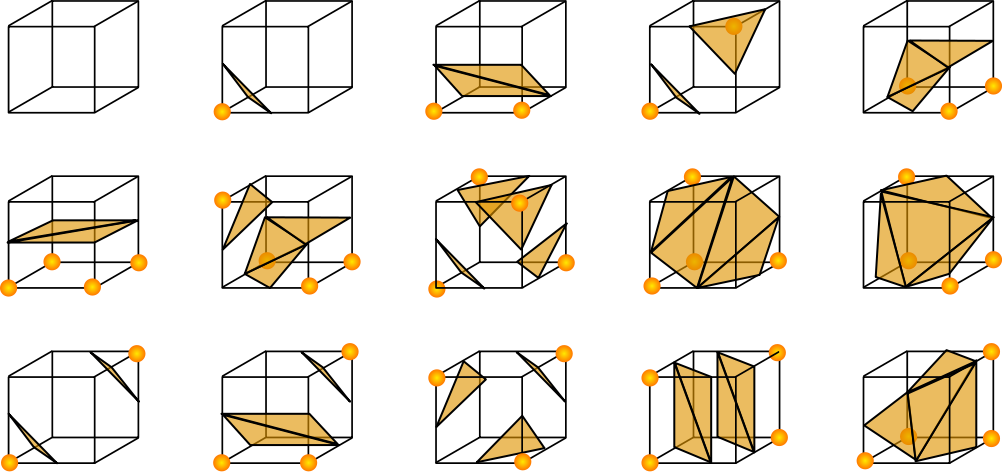
\includegraphics[scale=1.0]{img/cap01/mcCasos}
  \caption[Diferentes situaciones en el algoritmo de Marching Cubes]{Los diferentes casos de acuerdo a las configuraciones en MC. Los puntos amarillos se consideran interiores y donde no hay marca se consideran exteriores.}
  \label{fig:mcCasos}
\end{figure}

Para cada par $(\textbf{a}, \textbf{b})$ donde $\textbf{a}, \textbf{b} \in C(\textbf{k})$ tales que $v(\textbf{a}) > \tau$ y $v(\textbf{b}) \leq \tau$ y $(\textbf{a}, \textbf{b}) \in \omega$ se considera que el cruce de la superficie se encuentra en algún punto entre $\textbf{a}$ y $\textbf{b}$. El punto de cruce $\textbf{p}$ se puede hallar por interpolación lineal (aunque hay otros métodos \cite{mcResumen}) de la siguiente forma:
%En cada arista del cubo que posea un vértice interior (alternativamente exterior) y otro exterior (alternativamente interior) existe un cruce de la isosuperficie, por lo tanto se encuentra un vértice de un triángulo de $\mathcal{M}_{\tau}$. El lugar exacto del vértice en la arista puede estimarse por interpolación. En el MC estándar se hace una interpolación lineal de la siguiente forma, si una arista tiene extremos en $\textbf{k}_s$ y $\textbf{k}_e$, cuyos valores escalares son $v(\textbf{k}_s)$ y $v(\textbf{k}_e)$ respectivamente; entonces dado el isovalor $\tau$, el punto de intersección $\textbf{p}$ sobre la arista se puede encontrar con la siguiente formula: \begin{equation}
\begin{equation}
 \textbf{p} = \textbf{a} + \rho (\textbf{b} - \textbf{a}),
\label{ec:intepLineal}
\end{equation} en donde \begin{equation}
\rho = \dfrac{\tau - v(\textbf{a})}{v(\textbf{b}) - v(\textbf{a})}.
\label{ec:coefParaintepLineal}
\end{equation}

Una vez que se conocen todos los puntos de intersección en las aristas del cubo, se construyen los triángulos de las superficies de acuerdo al caso en el que se encuentre el cubo, ver Figura \ref{fig:mcCasos}. 

La colección de todas las caras triangulares $\mathcal{M}_{\tau}$, después de que el cubo ha recorrido todo el volumen, es la aproximación a la superficie $S_{\tau}$. Este algoritmo tiene la ventaja de que el hardware y el software para hacer gráficas por computadora es muy eficiente al dibujar triángulos. Además de que se puede saber fácilmente la normal a la superficie en cualquier punto de un triangulo (por ejemplo, calculando el producto vectorial de los segmentos que forman dos de sus lados).

\begin{figure}[htp]
 \centering
  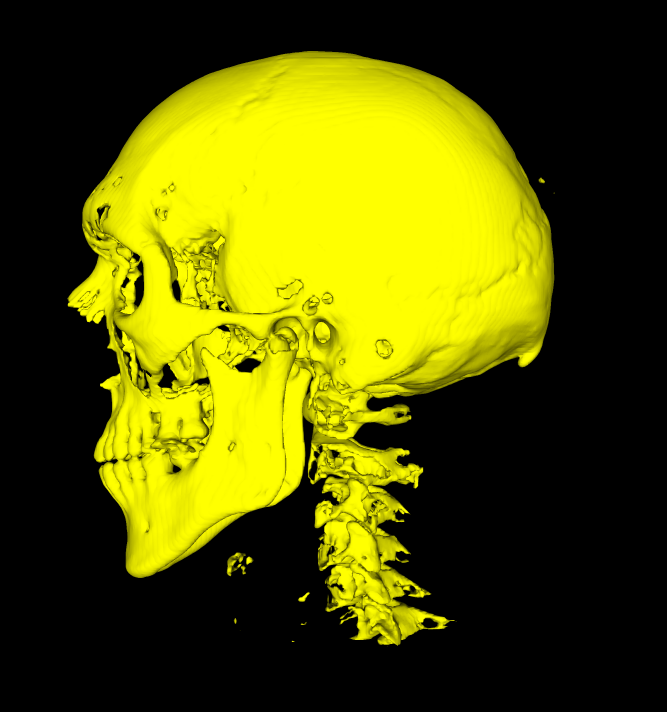
\includegraphics[scale=.45]{img/cap01/mc100}
  \caption[Ejemplo de superficie obtenida por Marching Cubes]{Superficie del mismo conjunto de datos de la Figura \ref{fig:imagenDigital} obtenida por Marching Cubes, para un isovalor $\tau = 100$.}
  \label{fig:ejmploMC}
\end{figure}

\subsection{El Algoritmo de seguimiento de superficies de Artzy}

Este fue uno de los primeros algoritmos que permite encontrar una aproximación a \eqref{ec:isosupeficie}. Fue propuesto por Ehud Artzy y por Gabor T. Herman en \cite{artzyCorto}. En su libro \cite{Gabor:DigitalSpaces} de posterior publicación, Herman usa el nombre de \emph{Algoritmo de Artzy} para referirse a este método.

Para usar este algoritmo necesitamos también un volumen $v$ junto con un umbral $\tau$. Su salida es también un conjunto de caras $\mathcal{A}_{\tau}$ que aproxima $S_{\tau}$, en este caso rectangulares y ortogonales a los ejes que definen $v$. A diferencia de MC este algoritmo necesita una entrada mas, una cara del conjunto $\mathcal{A}_{\tau}$ que sirve de posición de inicio (a veces llamada semilla).

\subsubsection{Condiciones del Algoritmo de Artzy}

El Algoritmo de Artzy empieza suponiendo que los vóxeles del volumen están de alguna manera clasificados en dos conjuntos: interior y exterior (conocido como un volumen binarizado). El criterio con el que se hace esta clasificación puede ser arbitrario. Por esto, el Algoritmo de Artzy puede usarse en conjunto con cualquier método de segmentación.

Dado que el propósito de este trabajo no es la segmentación (operación implícita en MC) y se desea ocupar el Algoritmo de Artzy como comparación con el algoritmo de MC, consideraremos todos los vóxeles $\textbf{k} \in \tau$ tales que $v(\textbf{k}) < \tau$ como exteriores y los vóxeles para los cuales $v(\textbf{k}) \geq \tau$ como interiores, para un cierto isovalor $\tau$. Este método de segmentación es conocido como umbralización.

Definimos tambien un elementos de la frontera o \emph{bel}, el término \emph{bel} viene del ingles \emph{boundary element}, como una cara común entre dos vóxeles $\omega$-adyacentes tales que uno de ellos es interior y el otro es exterior. Es fácil ver que para nuestros vóxeles los \emph{bels} serán caras rectangulares.

El Algoritmo de Artzy encuentra un conjunto $\mathcal{A}_{\tau}$ de caras de vóxeles tales que cada cara en $\mathcal{A}_{\tau}$ es un \emph{bel}. El conjunto $\mathcal{A}_{\tau}$ es la aproximación poligonal de la isosuperficie \eqref{ec:isosupeficie}. En términos mas concretos si $O$ es un conjunto de vóxeles interiores y $Q$ es un conjunto de vóxeles exteriores, definimos la frontera $\partial$ entre $O$ y $Q$ como:
\begin{equation}
\partial (O, Q) = \left\lbrace (\textbf{c}, \textbf{d}) | \textbf{c} \in O, \textbf{d} \in Q, \text{ y } (\textbf{c}, \textbf{d}) \in \omega \right\rbrace.
\label{ec:frontera}
\end{equation}

El Algoritmo de Artzy necesita un punto de inicio o semilla $\beta^0$. El punto de inicio es uno de los \emph{bels} $\in \partial (O, Q)$ y de ahí procede de manera iterativa hasta encontrar todos los \emph{bels} que aproximan la frontera $\partial(O, Q)$.

Para hacer este rastreo el algoritmo simplemente visita cada cara que sea un \emph{bel} de acuerdo a las rutas validas que se muestran en la Figura \ref{fig:artzyOrientacion}. La idea es que cada que se llega a una cara hay dos maneras de continuar de acuerdo a la orientación de la cara. Como las caras pertenecen a vóxeles cúbicos solo hay seis posibles orientaciones.

\begin{figure}[htp]
 \centering
  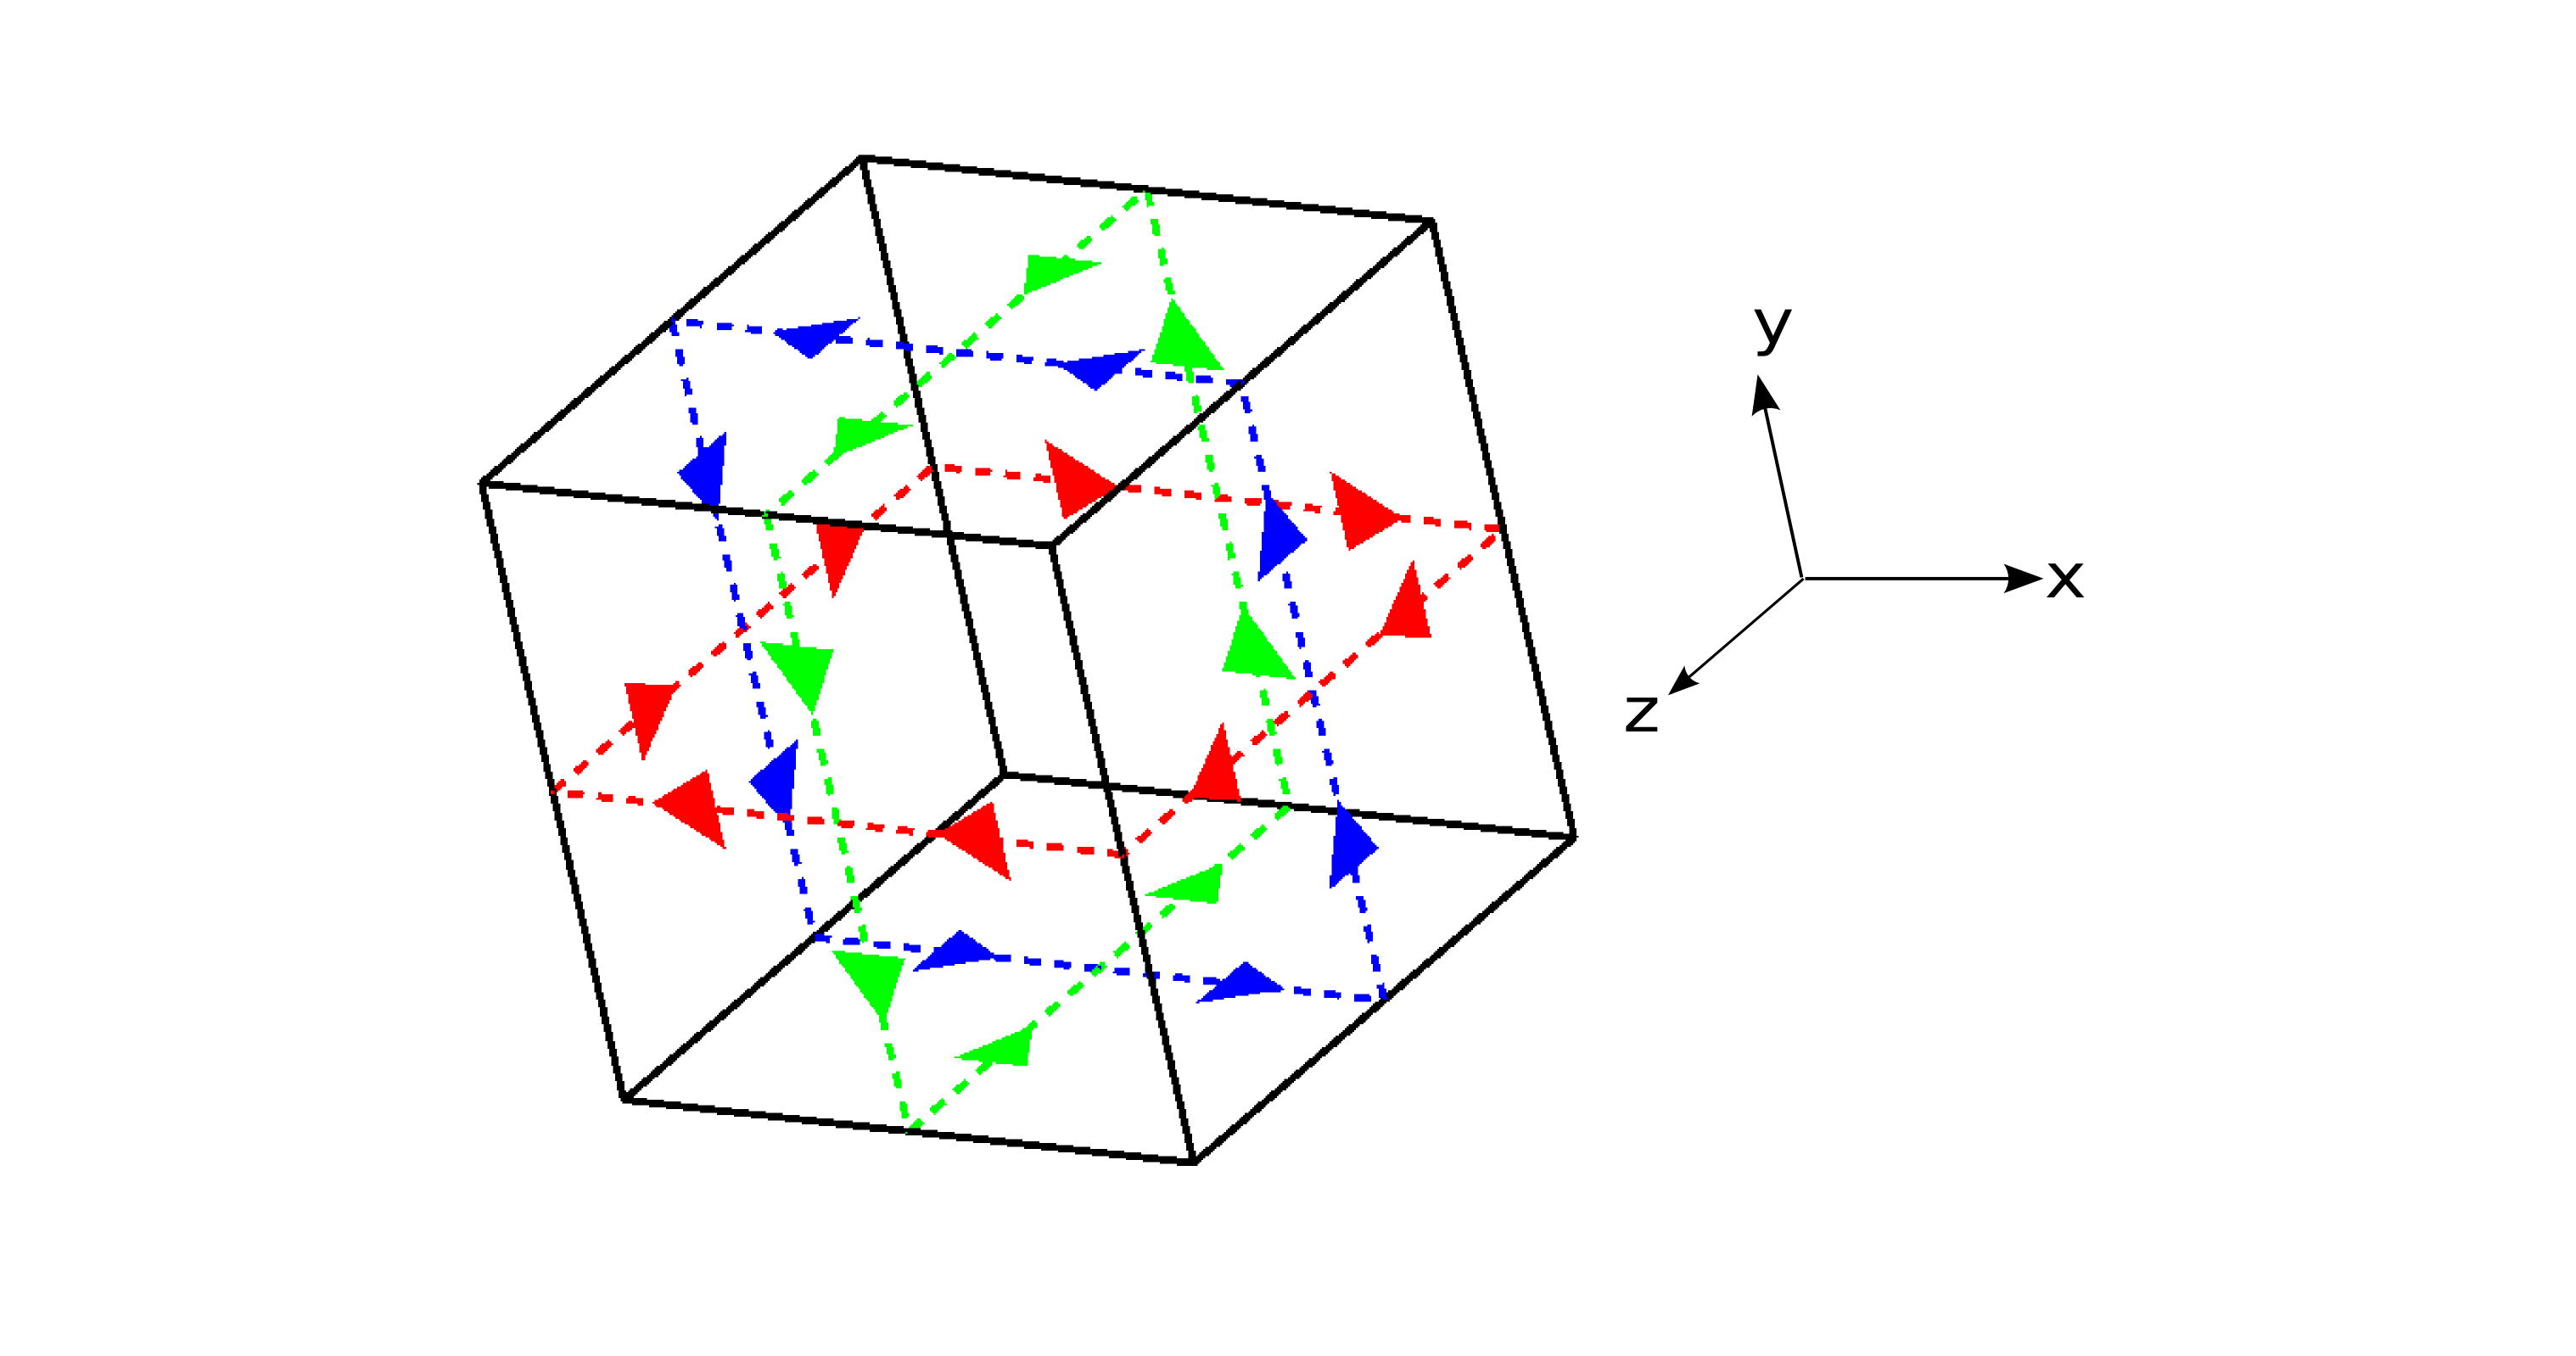
\includegraphics[scale=0.45]{img/cap01/artzyTrayectorias}
  \caption[Rutas validas en el Algoritmo de Artzy en la rejilla \textit{sc}]{En el Algoritmo de Artzy para cada cara hay dos formas validas de llegar y dos formas validas de salir.}
  \label{fig:artzyOrientacion}
\end{figure}

Cada vez que paramos en un \emph{bel} $\beta$ se toman las dos posibles direcciones válidas de salida y por cada una se busca una cara $\beta^i \in \partial$. Hay tres posibles casos ilustrados en la Figura \ref{fig:artzyCasos}. Supongamos que $\beta$ separa dos vóxeles $\textbf{a} \in O$ y $\textbf{b} \in Q$ y sean $\textbf{c}$ y $\textbf{d}$ los dos vóxeles tales que $(\textbf{b}, \textbf{c}) \in \omega$, $(\textbf{a}, \textbf{c}) \in \delta$, $(\textbf{b}, \textbf{d}) \in \delta$, $(\textbf{a}, \textbf{d}) \in \omega$ y que estan en la dirección valida a partir de $\beta$. Si $\textbf{c} \in O$ estamos en el caso ilustrado en la Figura \ref{fig:caso1Artzy}, si por el contrario $\textbf{c} \in Q$ debemos revisar en $\textbf{d}$. Si $\textbf{d} \in O$ estamos en el caso de la Figura \ref{fig:caso2Artzy} y si $\textbf{d} \in Q$ en el caso de la Figura \ref{fig:caso3Artzy}. En cualquiera de los casos anteriores siempre encontramos una cara $\beta^i \in \partial$.

%En la Figura \ref{fig:artzyCasos} se supone que estamos en la cara roja $\beta$ que es un \emph{bel}, que la dirección valida es apuntada por la flecha y se busca una posible cara azul $\beta_i$ que también sea un \emph{bel}. Como puede verse hay tres posibles casos, que dependen de si los vóxeles a la derecha y arriba de donde estamos son interiores o exteriores.

\begin{figure}[htp]
  \begin{center}
    \subfigure[Caso 1]{\label{fig:caso1Artzy}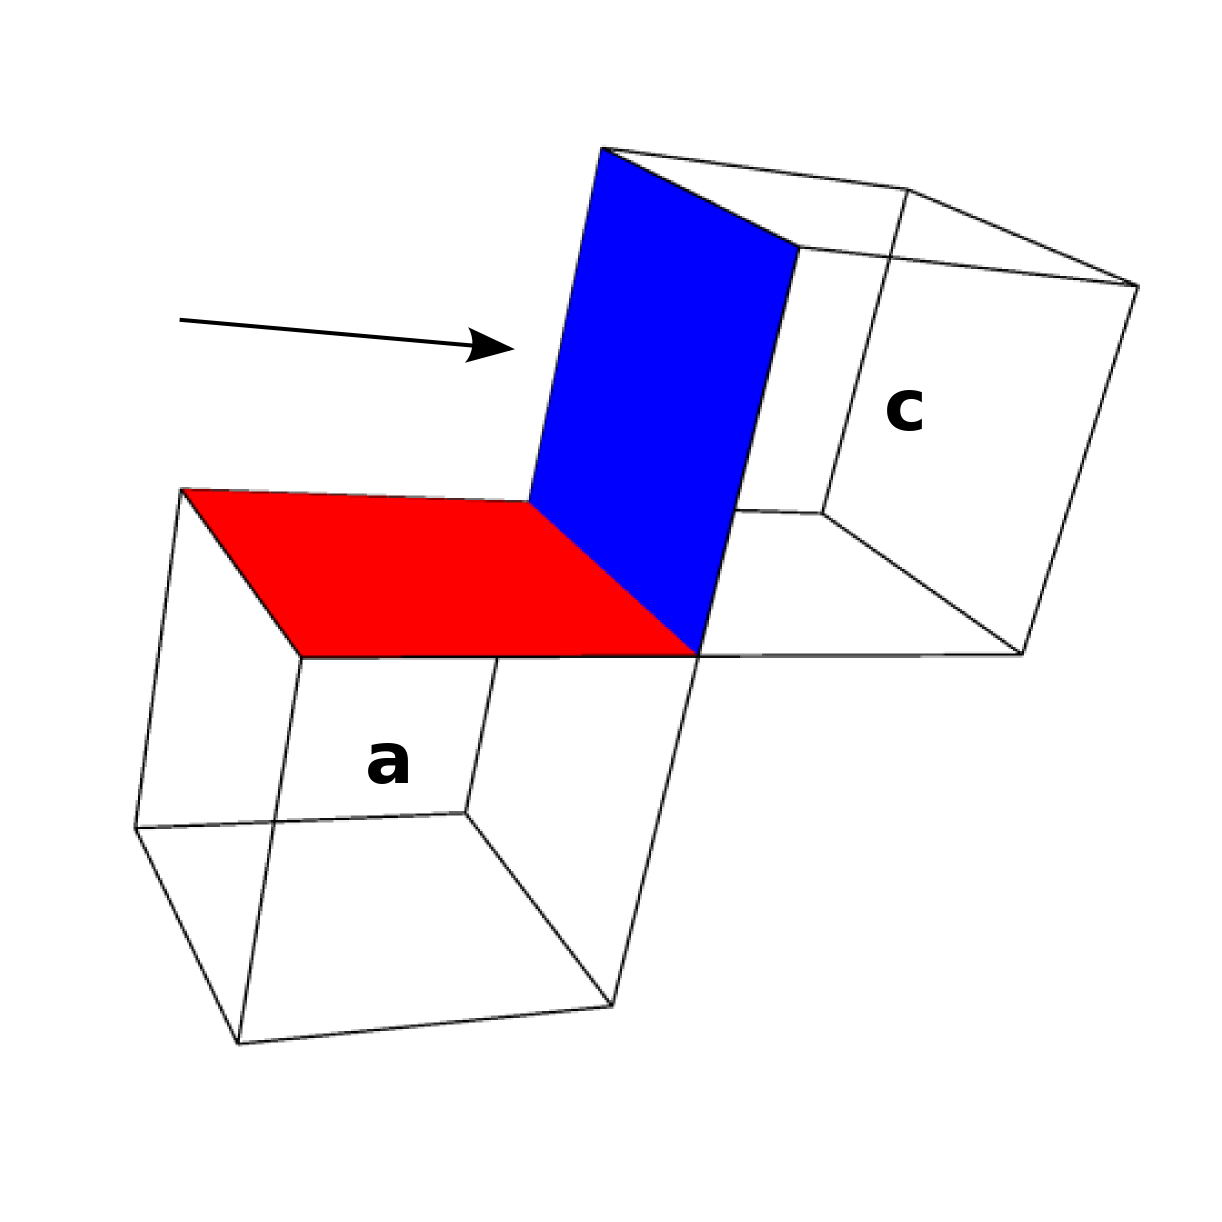
\includegraphics[scale=0.1]{img/cap01/caso1}}
    \subfigure[Caso 2]{\label{fig:caso2Artzy}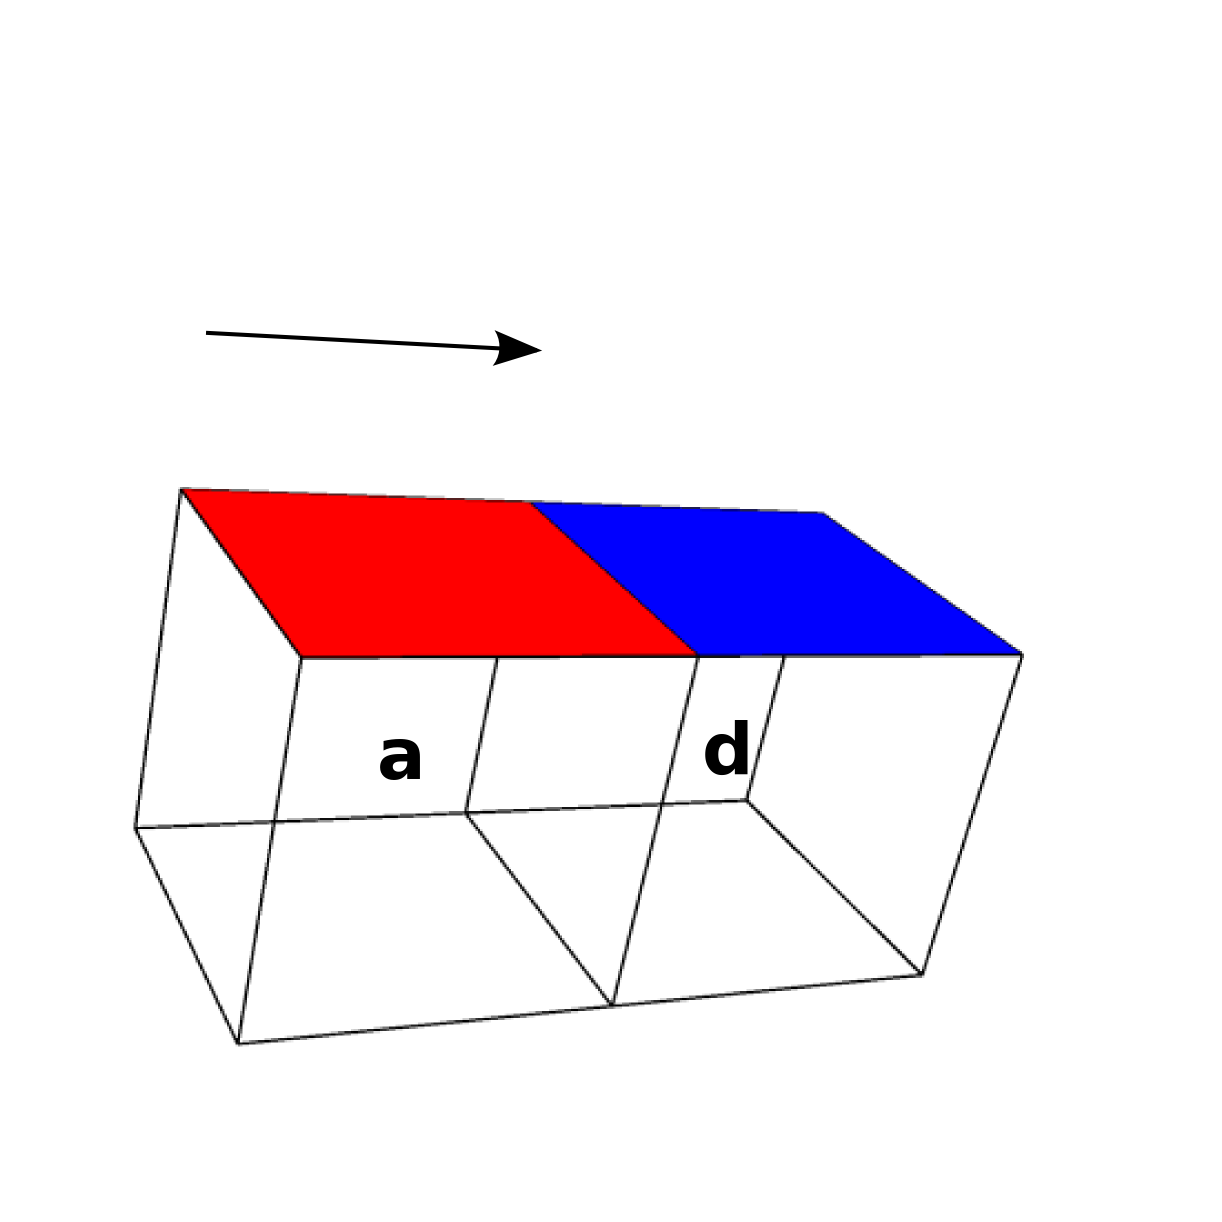
\includegraphics[scale=0.1]{img/cap01/caso2}}
    \subfigure[Caso 3]{\label{fig:caso3Artzy}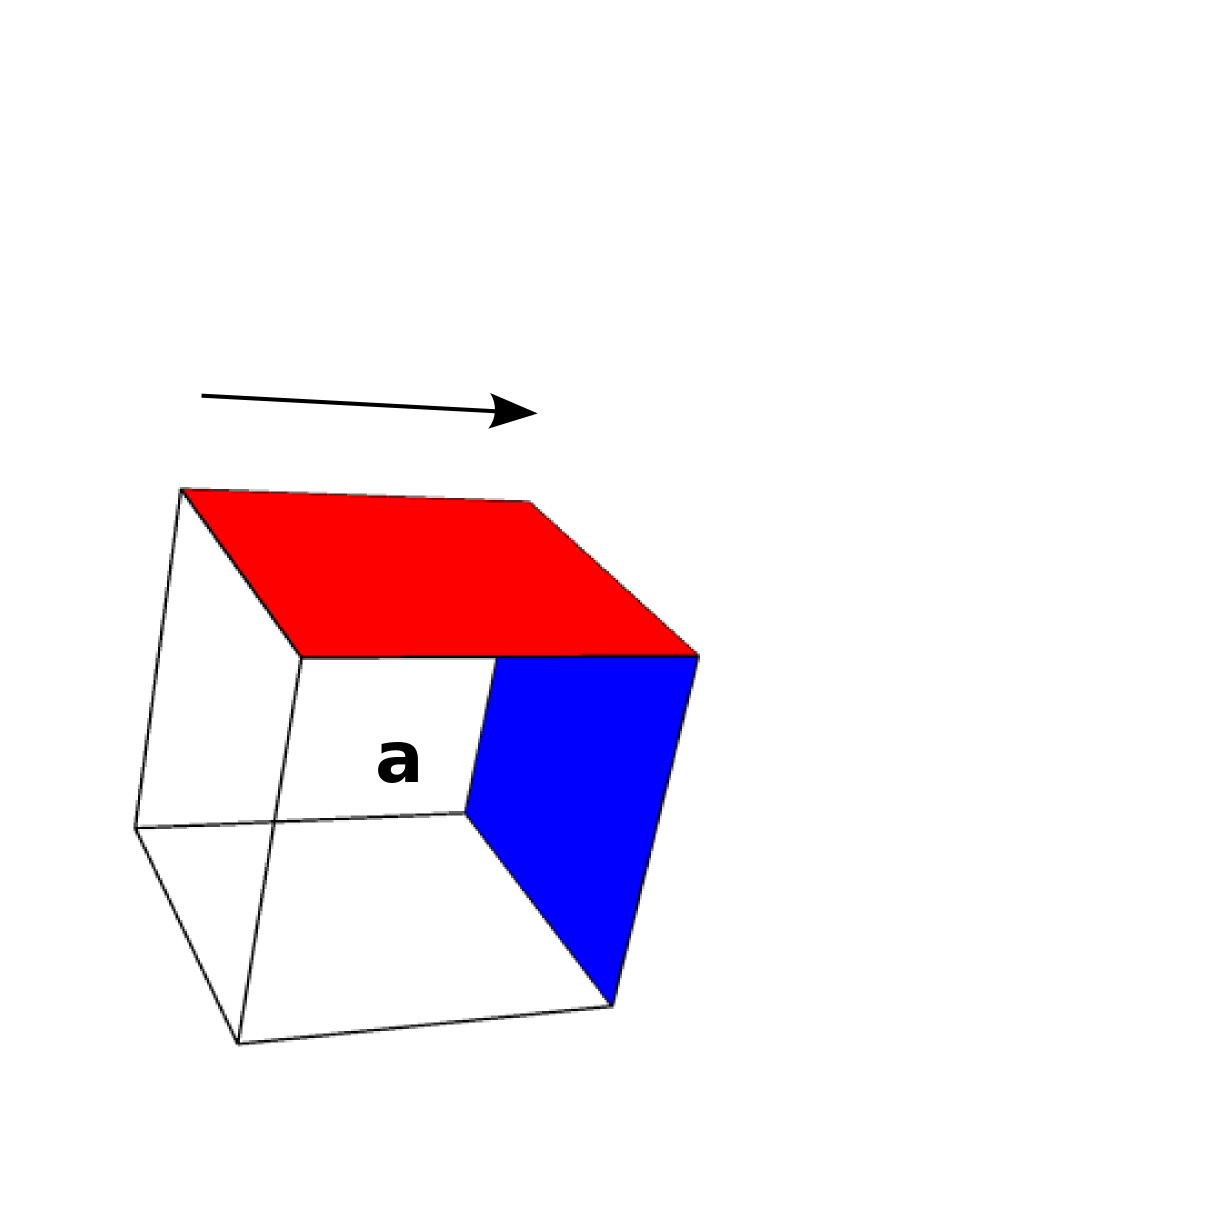
\includegraphics[scale=0.1]{img/cap01/caso3}} \\
  \end{center}
  \caption[Cambio de caras en el Algoritmo de Artzy]{Si se esta en la cara roja $\beta$ con la dirección valida apuntada por la flecha, hay tres casos posibles para encontrar la cara azul $\beta^i$. Por simplicidad en la figura solo se dibujan los vóxles en $O$.}
  \label{fig:artzyCasos}
\end{figure}

\subsubsection{Implementación del algoritmo}

En \cite{LargeSoftware} se realizó una implementación eficiente del Algoritmo de Artzy por medio de tres estructuras de datos:
\begin{itemize}
  \item Una lista auxiliar $L$ de caras $\beta$ que nos permita buscar en ella de manera eficiente. En la implementación se sugiere un árbol binario de búsqueda.
  \item Una cola $Q$ para tener un estado de espera donde guardar las rutas de salida validas que aun no se han recorrido. La lista $Q$ es una manera de simular el paralelismo que se define matemáticamente en \cite{Gabor:DigitalSpaces}. Debido a que se requiere que se exploren un número potencialmente grande de rutas al mismo tiempo este tipo de paralelismo no puede ser alcanzado en la implementación y debe simularse con una estructura de datos.
  \item La lista de \emph{bels} $\mathcal{A}_{\tau}$ que aproxima la superficie $S_{\tau}$.
\end{itemize}

El algoritmo se lista a continuación. Se asume que el volumen $v$, ha sido clasificado por algún criterio de segmentación para producir el volumen binarizado $B(v)$ y que de alguna manera se encontró un cara $\beta^0$ como semilla. En nuestra implementación se recorre $v$ vóxel por vóxel hasta que se encuentra la primera cara $\beta^{0}$ que se encuenta en la frontera definida en \eqref{ec:frontera}.

\begin{algorithm}[H]
\caption{Algoritmo de Artzy}
\label{algo:artzy}
\begin{algorithmic}[1]
\REQUIRE Un \emph{bel} inicial $\beta^0$ y el volumen binarizado $B(v)$.
\ENSURE Una lista $\mathcal{A}_{\tau}$ con todas las caras cuadradas que aproximan la superficie.
\STATE Colocar el \emph{bel} $\beta^0$ en la salida $\mathcal{A}_{\tau}$, agregar $\beta^0$ a $Q$ y poner dos copias de $\beta^0$ en $L$.
\WHILE{$Q \neq \emptyset$}
  \STATE Sacar una cara $\beta$ de $Q$
  \STATE Encontrar las caras $\beta^1$ y $\beta^2$ en $B(v)$ a las que se puede ir desde $\beta$, siguiendo las dos direcciones de la Figura \ref{fig:artzyOrientacion}, de acuerdo a alguno de los casos mostrados en la Figura \ref{fig:artzyCasos}.
  \IF{$\beta^1 \in L$}
    \STATE Quitar a $\beta^1$ de $L$
  \ELSE
    \STATE Agregar a $\beta^1$ en $\mathcal{A}_{\tau}$, en $L$ y en $Q$
  \ENDIF
  \IF{$\beta^2 \in L$}
    \STATE Quitar a $\beta^2$ de $L$
  \ELSE
    \STATE Agregar a $\beta^2$ en $\mathcal{A}_{\tau}$, en $L$ y en $Q$
  \ENDIF
\ENDWHILE

\end{algorithmic}
\end{algorithm}

\subsubsection{Propiedades del Algoritmo de Artzy}

Se demuestra en \cite{Gabor:DigitalSpaces} que el Algoritmo de Artzy es topológicamente correcto. Esto quiere decir de manera intuitiva que la frontera que produce es cerrada, conexa y que divide al espacio en dos. Es un análogo digital al Teorema de la Curva de Jordán \cite{Gabor:DigitalSpaces}.

Supongamos que el volumen $B(v)$ esta binarizado, supongamos también que conocemos una cara $\beta_0$ tal que está entre dos vóxeles $\textbf{g} \in O$, $\textbf{h} \in Q$ y $(\textbf{g}, \textbf{h}) \in \omega$. Sea también $O$ el componente $\delta$-conexo que contiene a $\textbf{g}$ y $Q$ el componente $\omega$-conexo que contiene $\textbf{h}$. El Algoritmo de Artzy asegura que después de un número finito de pasos tendremos a $\partial(O, Q) = \mathcal{A}_{\tau}$.

Aun más, asegura que esta frontera $\partial (O, Q)$ divide al espacio $\mathbb{Z}^3$ en dos subconjuntos propios $I$ y $E$, tales que:

\begin{enumerate}
  \item $O \subset I$ y $Q \subset E$.
  \item $\partial (O, Q) = \partial (I, E)$.
  \item $I \cup E = \mathbb{Z}^3$ y $I \cap E = \emptyset$.
  \item $I$ es un subconjunto $\delta$-conexo de $\mathbb{Z}^3$ y $E$ es un subconjunto $\omega$-conexo de $\mathbb{Z}^3$.
  \item Todo $\omega$-camino que vaya de un elemento de $I$ a un elemento de $E$ cruza $\partial (O, Q)$.
\end{enumerate}

La propiedad de mas importancia para nosotros es la última, pues nos asegura que a diferencia de MC, en el Algoritmo de Artzy nuestra aproximación poligonal a la isosuperficie $\mathcal{A}_{\tau}$ \emph{nunca} tiene agujeros.

La Figura \ref{fig:ejmploArtzy} presenta una superficie obtenida por el Algoritmo de Artzy, para el mismo conjunto de datos y con el mismo isovalor que el de la Figura \ref{fig:ejmploMC}.

\begin{figure}[htp]
 \centering
  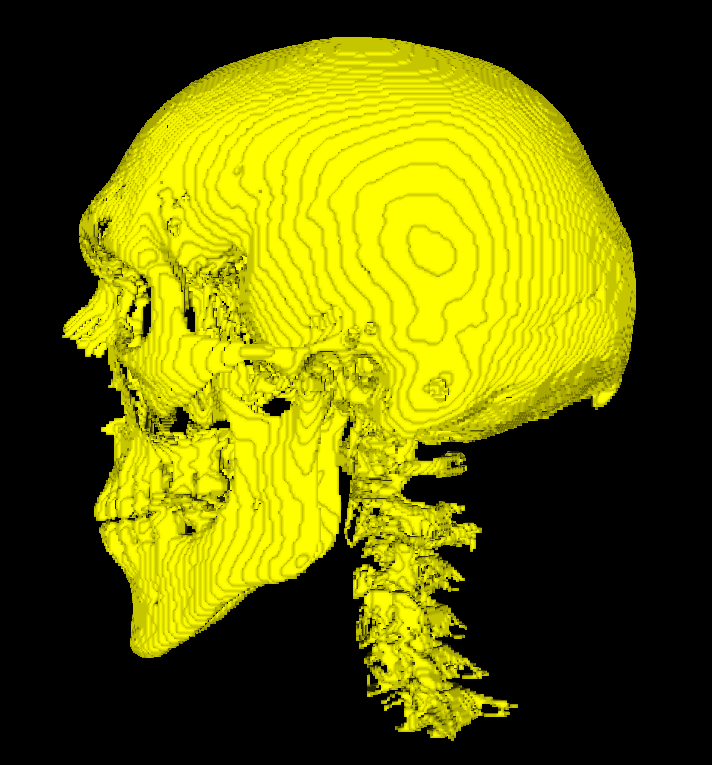
\includegraphics[scale=.45]{img/cap01/artzy}
  \caption[Ejemplo de superficie obtenida por el Algoritmo de Artzy]{Superficie obtenida por el Algoritmo de Artzy sobre el mismo conjunto de datos que en la Figura \ref{fig:ejmploMC} para un isovalor $\tau = 100$.}
  \label{fig:ejmploArtzy}
\end{figure}

\section{Visualización de mallas}
\label{sec:visualizarMallas}
Como mencionamos antes, una vez obtenida la aproximación a $S_{\tau}$ se utilizan técnicas de GC para producir una imagen 2D a partir del modelo, tratando de preservar la apariencia tridimensional.

El proceso por el que pasa la malla hasta producir la imagen final se conoce como \emph{render pipeline}. Durante este proceso se hacen operaciones que afectaran la apariencia de la imagen final. La técnicas que ayudan a conservar la apariencia tridimensional se les llama pistas de profundidad. Algunas de estas técnicas son las siguientes:

\begin{itemize}
  \item La \emph{proyección en perspectiva}. La proyección es la operación que proyecta el modelo 3D a un plano. Generalmente puede ser ortogonal o en perspectiva. En la proyección ortogonal los objetos no alteran su tamaño en función de la distancia al espectador. En contraste, en la proyección en perspectiva los objetos cambian su tamaño de acuerdo a la distancia a la que estén del espectador lo que da una apariencia mas cercana a la realidad.
  \item La \emph{eliminación de superficies ocultas}, también conocida en GC como \emph{z-buffering} o \emph{depth buffering} se encarga de eliminar las partes de objetos que se encuentran detrás de otros objetos en relación con el espectador. El efecto final consiste en que partes de algunos objetos de la escena no son visibles desde algunos puntos de vista.
  \item La \emph{iluminación} y el \emph{sombreado} son técnicas de GC que afectan en gran medida la imagen final. Consisten en modelar la interacción de la luz con los materiales de los que están hechos los objetos y por lo tanto dar una apariencia mas realista a la imagen final.
  \item El \emph{mapeo de texturas} y el \emph{mapeo de relieves} son técnicas que consisten en recalcular la apariencia de los píxeles finales en la imagen 2D con información guardada en un mapa y pueden afectar en gran medida la imagen final.
\end{itemize}


\subsection{Iluminación}

En graficación por computadora hay dos formas para poner color a una escena, una es simplemente asignándoles un color a los píxeles que están dentro de los objetos que es equivalente a decir que coloreamos los objetos. La otra consiste en calcular el color de cada píxel con base a las condiciones de iluminación en la escena.

La segunda de estas técnicas se conoce como iluminación y es visiblemente más agradable y realista que el coloreado. Para poder usar la iluminación es necesario definir fuentes de luz en la escena, luego definir las propiedades de reflectividad de los objetos, y también un vector normal unitario $\vec{\textbf{n}}$ a la superficie de los objetos.

La información de $\vec{\textbf{n}}$ se usa para dos cosas. La primera de ellas es determinar cual es la cara frontal del polígono, pues algunos dispositivos de despliegue en un intento por hacer el proceso mas rápido no dibujan la cara de atrás de los polígonos (esto se llama \emph{culling}). El segundo uso de $\vec{\textbf{n}}$ es para hacer cálculos de contribución de las luces en la escena a la iluminación del objeto.

El proceso de iluminación se lleva a cabo en dos partes, una donde se calcula la influencia de las luces en cada vértice del modelo de acuerdo con el modelo de iluminación (\emph{lighting model}) y otra donde se calcula el color de los píxeles que corresponden a los puntos en la superficie de cada polígono con base a un modelo de sombreado (\emph{shading model}).

%En este trabajo se analizan dos modelos de iluminación y dos modelos de sombreado: los modelos de iluminación son: el de Phong y el de Cook - Torrence. Y los modelos de sombreado son: el modelo de sombreado de Phong (diseñado para ser usado en conjunto con su modelo de iluminación) y el  de Gouraoud.

%En este trabajo se analizan dos modelos, uno de iluminación y uno de sombreado. El modelo de iluminación es el modelo de Phong y el modelo de sombreado es el modelo de Gouraud.

\subsubsection{Tipos de fuentes de luz}

Generalmente hay tres tipos de fuentes luz posibles que afectan la escena: las luces puntuales, las luces focales y las luces direccionales. Los diferentes tipos de fuente de luz están representados en la Figura \ref{fig:tiposLuz}.

\begin{figure}[htp]
  \begin{center}
    \subfigure[Luz direccional]{\label{fig:luzDirec}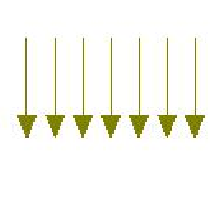
\includegraphics[scale=0.5]{img/cap01/luzDireccional}}
    \subfigure[Luz puntual]{\label{fig:luzPuntual}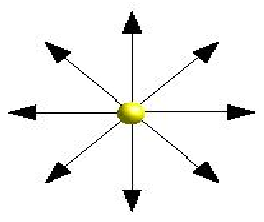
\includegraphics[scale=0.5]{img/cap01/luzPuntual}}
    \subfigure[Luz focal]{\label{fig:luzFocal}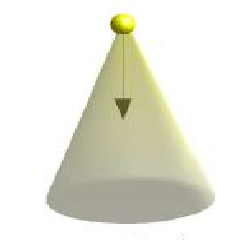
\includegraphics[scale=0.5]{img/cap01/luzFocal}} \\
  \end{center}
  \caption[Diferentes tipos de luz en una escena]{Tipos de fuentes de luz en una escena. Esta imagen fue tomada de \cite{libroCV}.}
  \label{fig:tiposLuz}
\end{figure}

\begin{description}
 \item[Luz direccional:] En este caso se asume que la fuente de luz está en el punto al infinito, por lo que a pesar de conocer la dirección en donde esta la fuente, ésta se encuentra tan lejos de la escena que los rayos de luz llegan de manera paralela.
\item[Luz puntual:] Se asume que la fuente de luz esta en un punto cercano e irradia sus rayos sobre la escena de manera igual en todas direcciones.
\item[Luz focal:] Éste es un caso particular del anterior, también sabemos la posición de la fuente de luz, pero ésta irradia sus rayos en una dirección preferente formando un cono de luz.
 \end{description}


\subsection{Modelos de iluminación}

El comportamiento físico de la luz es un fenómeno muy difícil de modelar. Por lo tanto, en las gráficas por computadora se usan modelos que aproximan este comportamiento de manera que los cálculos sean posibles en un tiempo razonable. Por esta razón se dice que los modelos de iluminación son \emph{inspirados en la física}, pero no son \emph{físicamente correctos} \cite{bussCG}.

\subsubsection{Modelo de Phong}

El modelo de iluminación de Phong es el mas usado actualmente, fue propuesto por Bui Tuong Phong en su tesis de doctorado \cite{Phong:Modelo}. Debido a su simpleza y los buenos resultados, se ha implementado eficientemente tanto en \emph{hardware} como en \emph{software}.

El modelo de Phong es en esencia un modelo de como se refleja la luz sobre los objetos en la escena. En este modelo se asume que el reflejo de la luz puede verse como la superposición de tres componentes independientes: la componente ambiental, la componente difusa y la componente especular. A su vez los objetos están hechos de cierto material. Cada material tiene una cierta sensibilidad a cada componente de la luz. De esta manera, cada material tiene coeficientes de reflexión ambiental, difuso y especular distintos. El color final de un píxel en el objeto en la escena es función del material y de las propiedades de la luces que interactúen con él.

Adicionalmente se asume que el modelo de percepción humana del color donde se percibe por medio de la superposición de tres longitudes de onda, llamados canales y que los cálculos de iluminación se pueden hacer en cada uno de los canales de manera independiente. Estos canales comúnmente representan luz en longitud de onda cercana al rojo, al verde y al azul. Por eso, la intensidad de la luz es representada como $\textbf{l} = (l_r, l_g, l_b)$ donde $l_r$,  $l_g$ y $l_b$ representan la longitud de onda cercana al rojo, al verde y al azul, respectivamente.

\subsubsection{La reflexión ambiental}

La reflexión ambiental es el color del objeto debido a los rayos de luz que provenían de una fuente, pero que han rebotado tantas veces en objetos de la escena que es imposible saber ni su dirección ni su origen. Se puede pensar que están flotando en la escena y llegan al objeto desde todas direcciones. Aun cuando en esta reflexión la luz parece estar en todas partes, desaparece si se apaga la fuente de donde proviene.

La reflexión ambiental $\textbf{r}_a$ se calcula en función de dos cosas. La luz que tiene un cierto componente ambiental $\textbf{l}_a$ y el objeto que reacciona con los rayos de luz de acuerdo a un coeficiente $0 \leq \rho_a \leq 1$. En el modelo de Phong se calcula como:
\begin{equation}
\textbf{r}_a = \rho_a \textbf{l}_a
\label{ec:refAmbiente}.
\end{equation}

\subsubsection{La reflexión difusa}

En esta reflexión los rayos de luz llegan al objeto provenientes de una fuente y al llegar son reflejados por la superficie del objeto en todas las direcciones posibles con la misma intensidad en cada dirección. Esta reflexión intenta modelar el comportamiento de la luz sobre superficies opacas. Véase la Figura \ref{fig:refDifusa} en donde la reflexión difusa se representa con flechas color naranja.

\begin{figure}[htp]
 \centering
  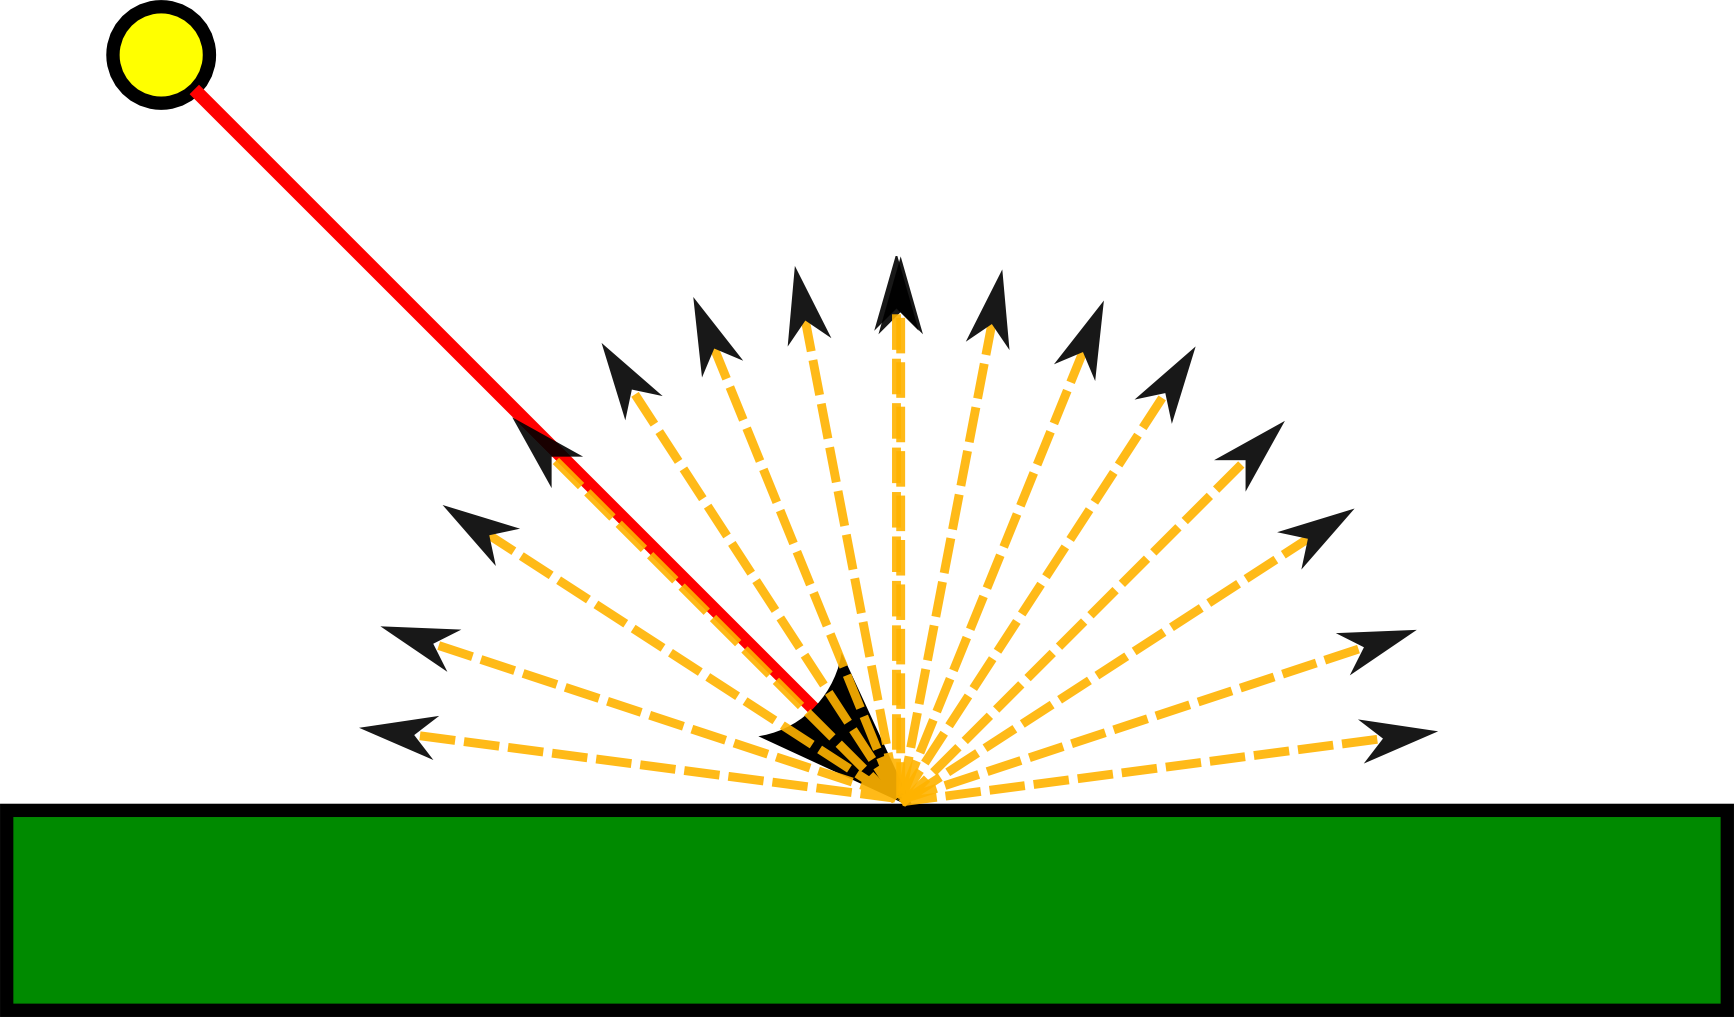
\includegraphics[scale=1.0]{img/cap01/difusa}
  \caption[Reflexión difusa]{El rayo de luz rojo incide en la superficie y es reflejado en todas las direcciones posibles.}
  \label{fig:refDifusa}
\end{figure}

La reflexión difusa es función de cuatro cosas. Primero las propiedades de la fuente de luz $\textbf{l}_d$. Luego la posición relativa de la fuente de luz con respecto al punto donde estemos calculando la iluminación. Tercero, el coeficiente de reflexión difusa $0 \leq \rho_d \leq 1$ específico al material del objeto. Por último el vector normal $\vec{\textbf{n}}$ a la superficie del objeto en el punto donde estemos calculando la iluminación.

El modelo de Phong modela la reflexión difusa de la siguiente manera:

\begin{equation}
\textbf{r}_d = \rho_d \textbf{l}_d (\textbf{c} \cdot \vec{\textbf{n}}), 
\label{ec:refDifusa}
\end{equation}
en donde $\textbf{c} = \textbf{l} - \textbf{p}$ es un vector que va del punto donde estamos calculando la iluminación a la fuente de luz, ver la Figura \ref{fig:phongGeo}.

\subsubsection{La reflexión especular}

Aquí los rayos de luz llegan al objeto y son reflejados por la superficie de éste en una dirección preferente, ver Figura \ref{fig:refEspecular}. Esta reflexión intenta modelar la interacción de la luz con superficies muy brillantes. El espectador sólo percibe esta reflexión si esta en algún lugar a donde lleguen los rayos reflejados y mientras más se acerca al reflejo perfecto más intensa es para él esta reflexión.

\begin{figure}[htp]
 \centering
  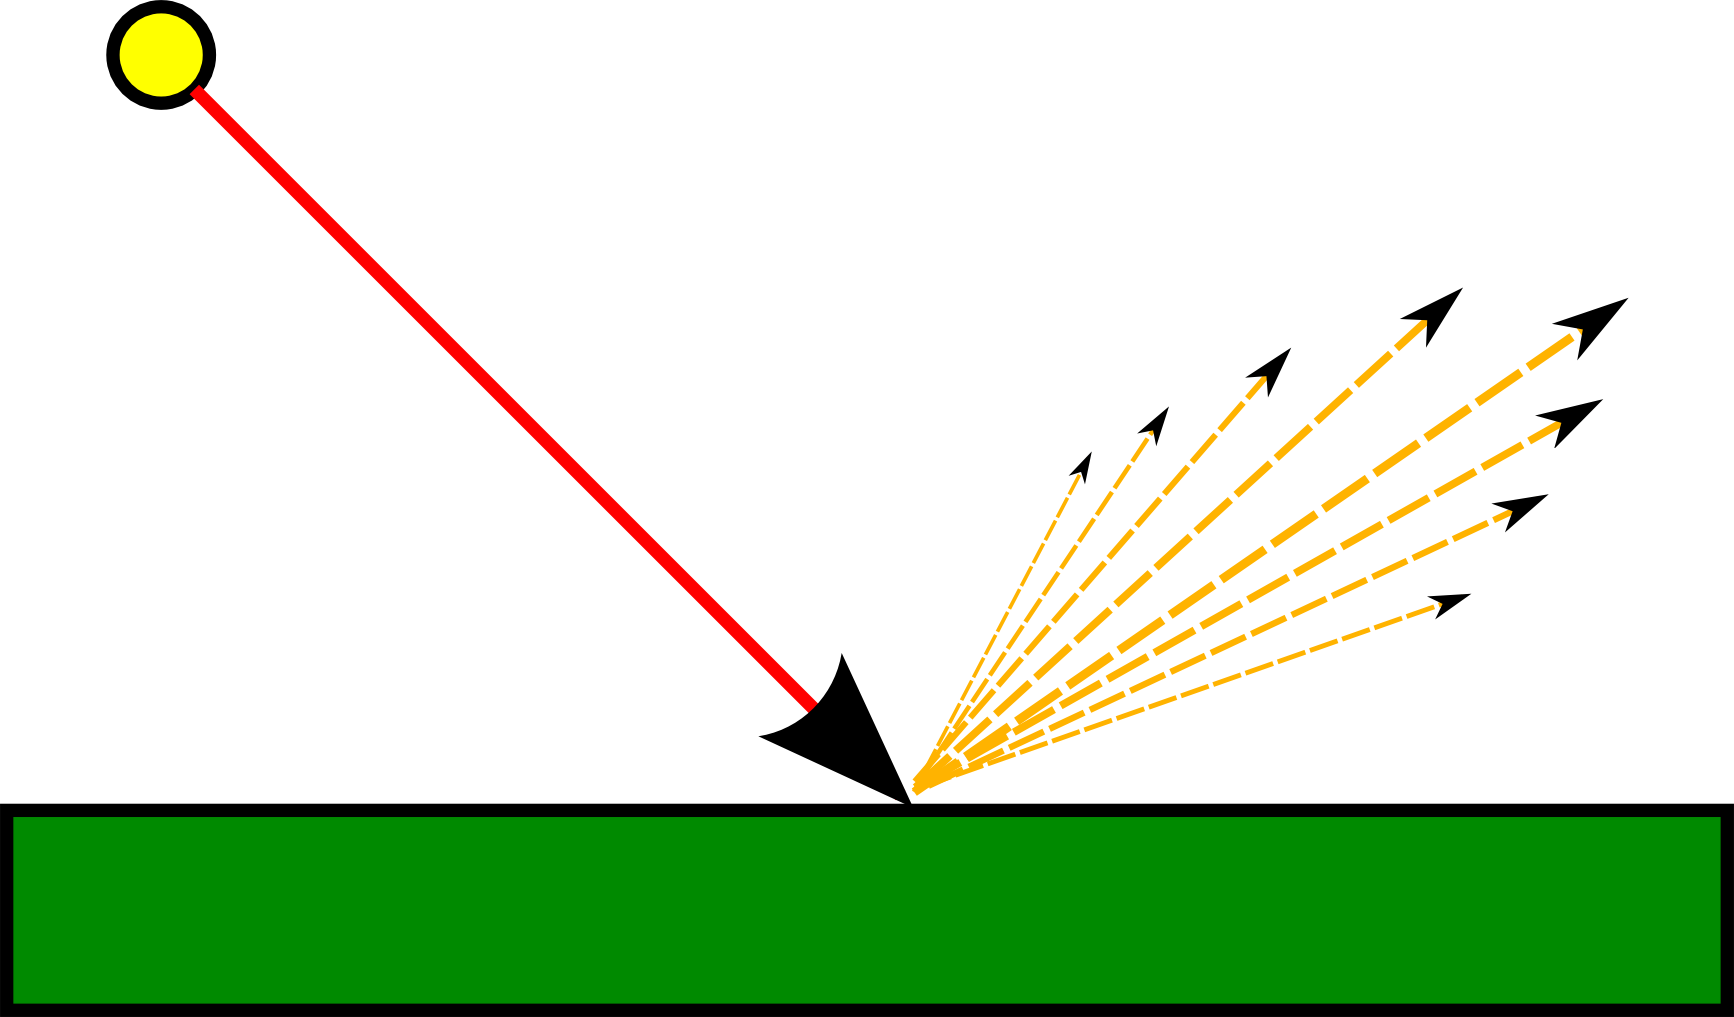
\includegraphics[scale=1.0]{img/cap01/especular}
  \caption[Reflexión especular]{El rayo de luz rojo incide en la superficie y es reflejado en una dirección preferente.}
  \label{fig:refEspecular}
\end{figure}

La reflexión especular en este modelo se calcula con la siguiente fórmula
\begin{equation}
\textbf{r}_s = \rho_s \textbf{l}_s (\textbf{d} \cdot \textbf{e})^\gamma, 
\label{ec:refEspecular}
\end{equation}
en donde $\textbf{e}$ es un vector del punto que estamos calculando a la posición del observador. El vector $\textbf{d}$ va del punto donde estamos calculando a donde se haría el reflejo perfecto del rayo proveniente de la fuente de luz. El coeficiente $0 \leq \rho_s \leq 1$ es una propiedad del material del objeto, al igual que el parámetro $\gamma \geq 0$ que dice que tan brillante es el objeto. Todo puede verse en la Figura \ref{fig:phongGeo}.

\begin{figure}[htp]
 \centering
  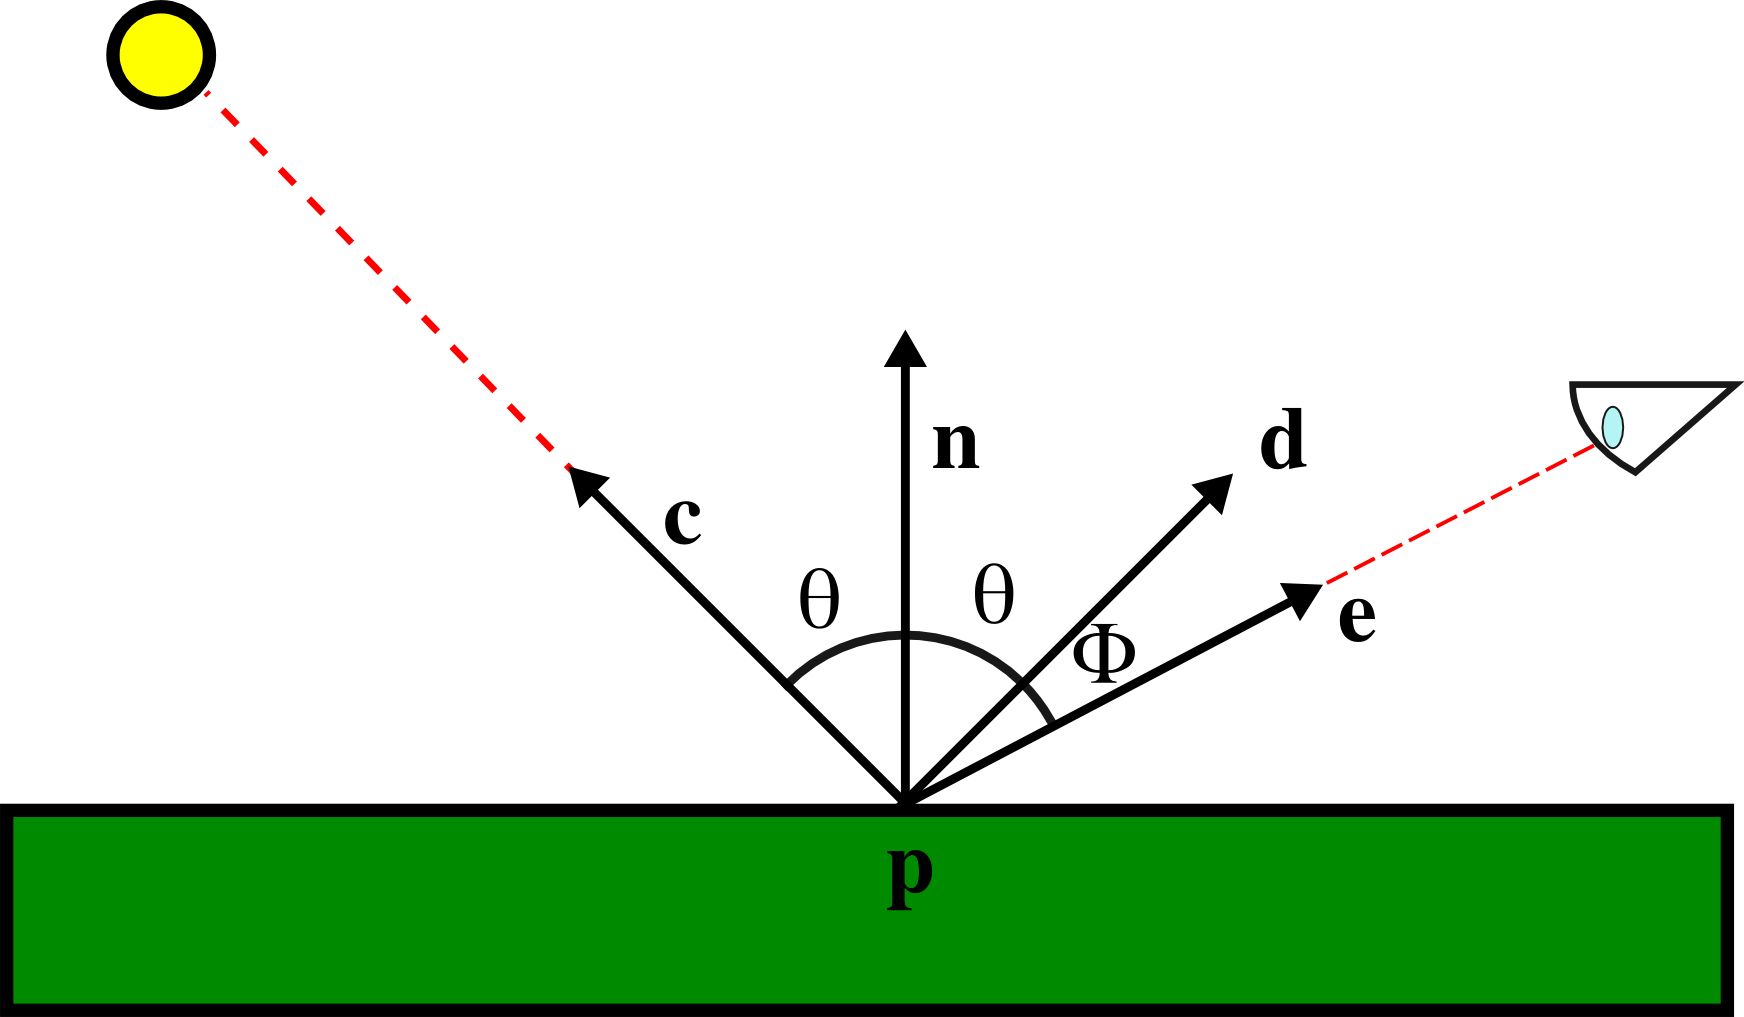
\includegraphics[scale=1.0]{img/cap01/geometria}
  \caption[Situación geométrica del modelo de Phong]{La situación geométrica del modelo de Phong. El circulo amarillo es la fuente de luz y el ojo el observador.}
  \label{fig:phongGeo}
\end{figure}

El vector $\textbf{d}$ es aquel vector coplanar con $\vec{\textbf{n}}$ y con $\textbf{c}$ que hace el mismo ángulo $\theta$ con $\vec{\textbf{n}}$ que $\textbf{c}$ y puede calcularse $\textbf{d} = 2(\textbf{c} \cdot \vec{\textbf{n}})\vec{\textbf{n}} - \textbf{c}$. El ángulo $\Phi$ entre los vectores $\textbf{d}$ y $\textbf{e}$ nos dice que tan cerca estamos del reflejo perfecto. Mientras el parámetro $\gamma$ sea mas grande el abanico del reflejo especular es más angosto (Figura \ref{fig:refEspecular}), valores típicos de $\gamma$ van en el rango $[50, 80]$.

\subsubsection{Modelo completo}

En el modelo de Phong se asume que los componentes de cada reflexión son independientes, por lo tanto el color final $\textbf{l}$ de cada píxel se puede obtener sumando las reflexiones de cada componente 
\begin{equation}
\textbf{l} = \textbf{r}_a + \textbf{r}_d + \textbf{r}_s. 
\label{ec:phongModelunaLuz}
\end{equation}

En la Figura \ref{fig:ejemPhongComp} se pueden ver los efectos y contribuciones de este modelo. Donde primero se presentan los efectos de cada reflexión por separado y luego se presentan todos los componente juntos.

\begin{figure}[htp]
  \begin{center}
    \subfigure[Reflexión ambiental]{\label{fig:ejemAmb}
\includegraphics[scale=0.3]{img/cap01/reflexionAmbiente}}
    \subfigure[Reflexión difusa]{\label{fig:ejemDif}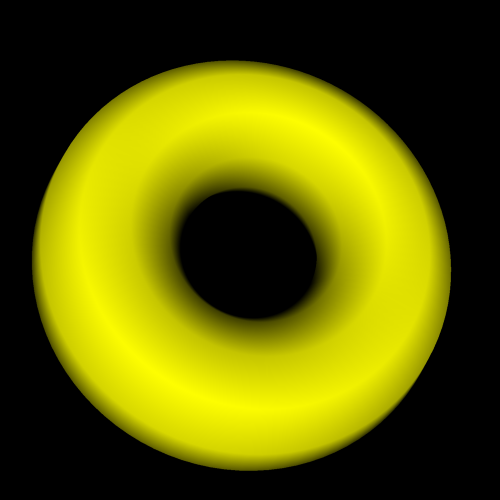
\includegraphics[scale=0.3]{img/cap01/reflexionDifusa}} \\
    \subfigure[Reflexión especular]{\label{fig:ejemEspe}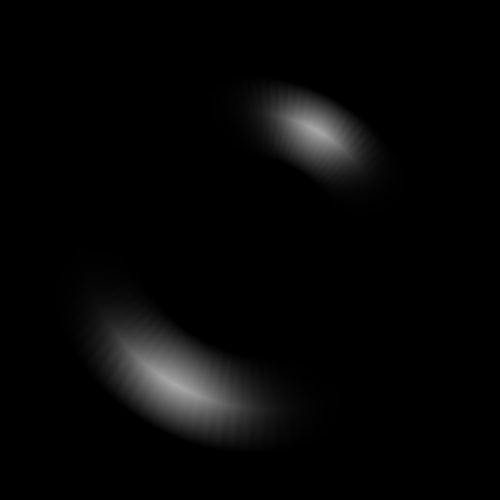
\includegraphics[scale=0.3]{img/cap01/reflexionEspecular}}
    \subfigure[Modelo completo]{\label{fig:ejemPhong}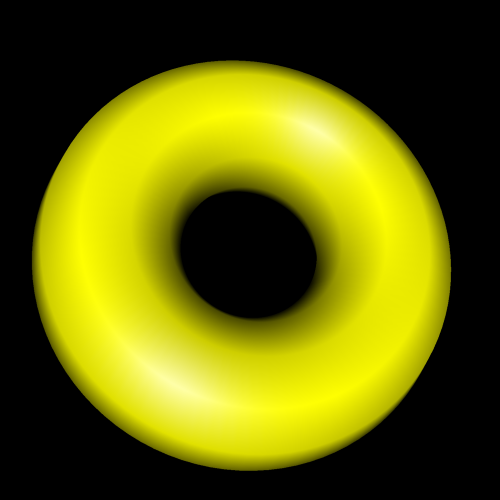
\includegraphics[scale=0.3]{img/cap01/modeloCompleto}}
  \end{center}
  \caption[Componentes del modelo de iluminación de Phong]{Componentes del modelo de iluminación de Phong.}
  \label{fig:ejemPhongComp}
\end{figure}

Hasta ahora los cálculos se han hecho bajo la suposición de que hay solo \emph{una} luz afectando en la escena en caso de haber mas de una luz se suman las contribución de cada luz sobre el punto donde se este calculando la iluminación. También es común tener una componente ambiental $\textbf{r}_{a}^{g} = \rho_a \textbf{l}^{g}$ que representa una contribución en el componente ambiental de la escena misma, es decir que no se debe a ninguna luz. Por lo que en una escena donde hay $L$ luces el color del píxel es
\begin{equation}
\textbf{l} = \sum_{i = 1}^{L} \left( \textbf{r}_{a}^{i} + \textbf{r}_{d}^{i} + \textbf{r}_{s}^{i} \right) + \textbf{r}_{a}^{g}
\label{ec:phongModelo}
\end{equation}

Hay que tener cuidado al usar la ecuación anterior. Antes de sumar la contribución de cada luz debemos ver que ésta de verdad ilumine al punto donde estamos calculando la iluminación. Debemos verificar que $\vec{\textbf{n}} \cdot \textbf{c}^{i} > 0$ en caso contrario simplemente saltamos esa contribución sin hacer ningún calculo. Físicamente si $\vec{\textbf{n}} \cdot \textbf{c}^{i} \leq 0$ significa que la luz y el punto a iluminar están en lados opuestos de la superficie, como puede deducirse de la Figura \ref{fig:phongGeo}.

Se hace énfasis de que en éste modelo las reflexiones que mas contribuyen al efecto final de la escena son la especular y la difusa (ver la Figura \ref{fig:ejemPhongComp}), las cuales son funciones del vector normal $\vec{\textbf{n}}$.

\subsection{Modelos de sombreado}

El modelo de iluminación se encarga de calcular el color de los vértices de la malla. Sin embargo, para hacer el despliegue esto no es suficiente, pues generalmente queremos desplegar los polígonos que forman la malla y necesitamos conocer el color en todos los puntos interiores del polígono no solo en su vértice. A la acción de calcular el color que deben tener los puntos interiores de un polígono en función de los colores de los vértices se le llama \emph{sombreado} (en ingles el término es \emph{shading}).

El sombreado se lleva a cabo en la última etapa del render pipeline llamada \emph{rasterización} \cite{redBook}. Esta etapa, a diferencia del resto del render pipeline es dependiente del \emph{hardware} de despliegue. Para hacer la rasterización es necesario transformar todo el modelo de coordenadas en números reales a una discretización en coordenadas enteras que se corresponden con los píxeles del dispositivo de despliegue\cite{shadersBook}. Debido a que el interior del polígono tiene puntos infinitos no podemos hacer el cálculo si no hasta saber cuales de estos puntos se verán en la imagen final. Es decir, necesitamos saber cuales de los puntos del polígono corresponderán a píxeles en el dispositivo de salida y solo se hacen los cálculos en estos puntos.

Los algoritmos de raster solo son capaces de actuar sobre triángulos debido a que necesitan asegurarse que el polígono a colorear es plano y convexo. En etapas anteriores del render pipeline los polígonos que forman el modelo son triangulados. De esta manera, aunque el modelo estuviera originalmente compuesto de polígonos complejos, al rasterizador solo llegan triángulos.

Para hacer su trabajo el rasterizador sabe las coordenadas y el color de los vértices de cada triángulo. Hace una correspondencia de cada vértice al píxel mas cercano de manera que tiene la situación representada en la Figura \ref{fig:lineScan}.

\begin{figure}[htp]
 \centering
  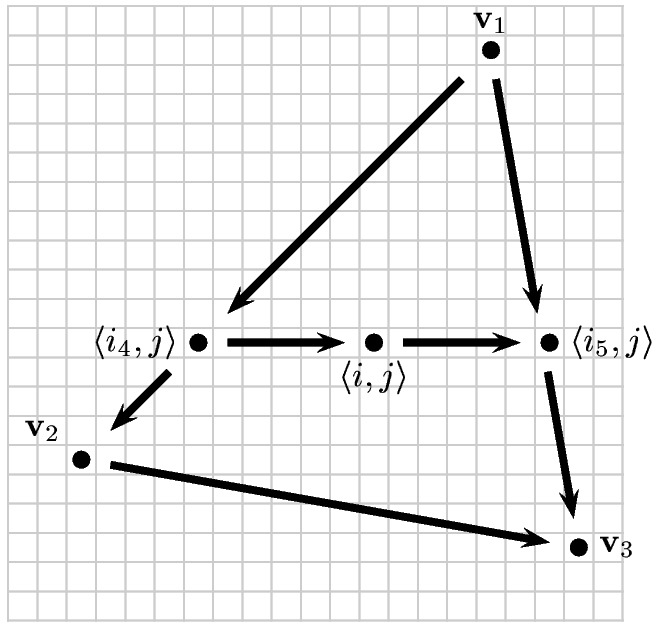
\includegraphics[scale=0.4]{img/cap01/lineScan}
  \caption[Ejemplo de sombreado sobre un triangulo]{El algoritmo de \emph{line scan} calcula el color de los píxeles interiores del triángulo. Esta imagen fue tomada de \cite{bussCG}.}
  \label{fig:lineScan}
\end{figure}

El algoritmo de \emph{raster} mas común es conocido como \emph{line scan}. El primer paso del algoritmo consiste en calcular que píxeles forman las aristas del triangulo. Para calcular los píxeles que forman cada una de las aristas se hace uso del algoritmo de Bresenham \cite{bresenhamAlgorithm}. Después el algoritmo calcula el color de los píxeles de cada arista usando el color de los vértices. Por último el algoritmo empieza a barrer de manera horizontal todos los píxeles interiores del triangulo (de aquí su nombre) en cada píxel calcula el color entre los colores de los vértices que estén al inicio y al final del segmento horizontal sobre el que esta barriendo. En la Figura \ref{fig:lineScan} se muestra el cálculo del color del píxel $\langle i, j\rangle$ en función de los colores de los píxeles $\langle i_4, j\rangle$ y $\langle i_5, j\rangle$. 

\subsubsection{Sombreado de Gouraud}
Para que el algoritmo de \emph{raster} funcione, necesita calcular los colores de los píxeles de un segmento de recta en función de los colores en los puntos extremos del segmento que lo delimitan. La manera como se hace este cálculo es dependiente del modelo de sombreado. El modelo de sombreado mas usado es el de Gouraud, que fue propuesto en \cite{gouraudShading}.

El sombreado de Gouraud es muy usado por su gran facilidad, actualmente esta implementado tanto en \emph{software} como en \emph{hardware} en las tarjetas gráficas. Básicamente consiste en hacer una interpolación lineal de los colores de los píxeles en las aristas a partir del color de los vértices del triángulo. Luego, hacer interpolación lineal para calcular el color de los píxeles interiores del triangulo a partir de los colores recién calculados en las aristas. Esto se conoce mas generalmente como \emph{interpolación bilineal}.

Dicho de otra manera si en un segmento de recta los limites $\textbf{x}_0$ y $\textbf{x}_1$ tienen colores $\langle r_0, g_0, b_0 \rangle$ y $\langle r_1, g_1, b_1 \rangle$ y algún otro píxel está posicionado sobre el segmento de recta a una fracción $\rho$ del camino que va de $\textbf{x}_0$ a $\textbf{x}_1$, su color debería ser
\begin{equation}
  (1 - \rho) \langle r_0, g_0, b_0 \rangle + \rho \langle r_1, g_1, b_1 \rangle.
 \label{ec:gouraudShading}
\end{equation}

Como ejemplo, haciendo referencia de nuevo a la Figura \ref{fig:lineScan} primero interpolamos linealmente los colores del segmento que va de $\textbf{v}_1$ a $\textbf{v}_2$ (en algún momento de este paso calculamos el color en $\langle i_4, j\rangle$), luego calculamos de la misma manera los colores del segmento de $\textbf{v}_1$ a $\textbf{v}_3$ (entre éstos al color de $\langle i_5, j\rangle$) y finalmente de $\textbf{v}_2$ a $\textbf{v}_3$. Luego procedemos a calcular los colores en el interior del triángulo, entre estos calculamos el color de $\langle i, j\rangle$.

Una de las desventajas importantes del modelo de Gouraud es que si un efecto luminoso, por ejemplo una reflexión especular, debería de afectar los píxeles interiores de un triangulo, pero por la situación geométrica no afecta ninguno de los vértices del mismo triangulo, entonces el sombreado de Gouraud pierde ese efecto luminoso.

\subsubsection{Sombreado de Phong}

En \cite{Phong:Modelo} no solo se propone un modelo de iluminación si no también se propone un modelo de sombreado para usarse en conjunto con el modelo de iluminación. Aunque este modelo fue diseñado para usarse en conjunto con el modelo de iluminación de Phong y proporciona mejores resultados que el modelo de Gouraud, en muchas aplicaciones se prefiere no usarlo debido a que requiere hacer cálculos considerablemente mas complicados.

En éste modelo se hace uso de la interpolación bilineal exactamente como la antes descrita, pero en vez de interpolar los colores, se interpolan las normales. Como las normales para la iluminación deben ser unitarias si existen dos píxeles  $\textbf{x}_0$ y $\textbf{x}_1$ donde las normales son $\textbf{n}_0$ y $\textbf{n}_1$ respectivamente, en un píxel que está a fracción $\rho$ de $\textbf{x}_0$ en el segmento de $\textbf{x}_0$ a $\textbf{x}_1$, la normal interpolada es:

\begin{equation}
  \dfrac{(1 - \rho)\textbf{n}_0 + \rho \textbf{n}_1}{\lVert (1 - \rho)\textbf{n}_0 + \rho \textbf{n}_1 \rVert}.
  \label{ec:phongShading}
\end{equation}

Una vez que se conoce la normal, el color del píxel se calcula usando de nuevo el modelo de iluminación descrito en \eqref{ec:phongModelo}. Por esta razón, es necesario que información acerca de la posición y color de las luces, además del material del objeto se conserve en el pipeline hasta la etapa de rasterizado. 

En éste modelo se corrige la desventaja de Gouraud explicada anteriormente. En contraste, una de las desventajas de usar el modelo de Phong son la mayor cantidad de cálculos y la necesidad de guardar mas información durante todo el render pipeline. Sin embargo, actualmente con las nuevas tarjetas de video esto no es un factor determinante.

Otra de las desventajas de interpolar linealmente las normales de una malla es la tasa de cambio de las normales. En polígonos que estén orientados frente al espectador las normales cambiaran mas lentamente que en áreas donde las normales estén apuntando hacia los lados del espectador.

Una manera de compensar este problema es usar las siguientes fórmulas para calcular las normales:

\begin{eqnarray}
  \nonumber
  n_{1}(\rho) & = (1 - \rho)n_{1,0} + \rho n_{1, 0}, \\
  \nonumber
  n_{2}(\rho) & = (1 - \rho)n_{2,0} + \rho n_{2, 0}, \\
  n_{3}(\rho) & = \sqrt{1 - n_{1, \rho}^{2} - n_{2, \rho}^{2}}.
  \label{ec:phongShadingCorrection}
\end{eqnarray}

Una comparación entre sombrear con el modelo de Phong y con el modelo de Gouraud se puede ver en la Figura \ref{fig:shadingComparation}.
\begin{figure}[htp]
  \begin{center}
    \subfigure[Sombreado de Gouraud]{\label{fig:gouraudShading}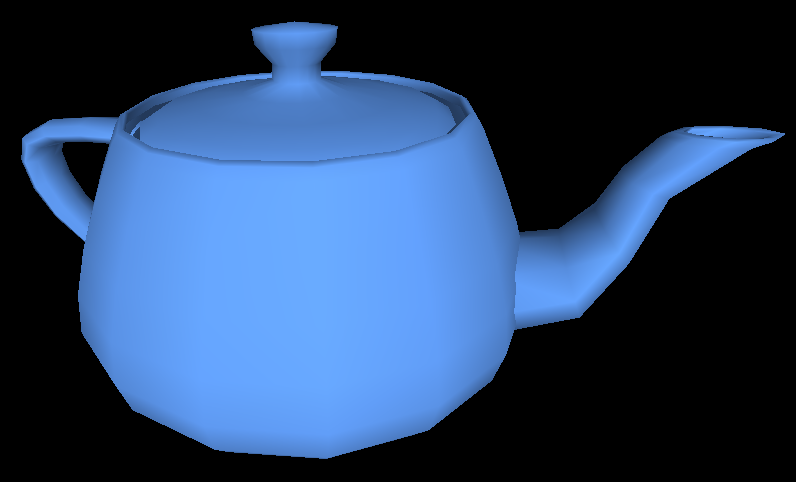
\includegraphics[scale=0.35]{img/cap01/teapotGouraud}}
    \subfigure[Sombreado de Phong]{\label{fig:phongShading}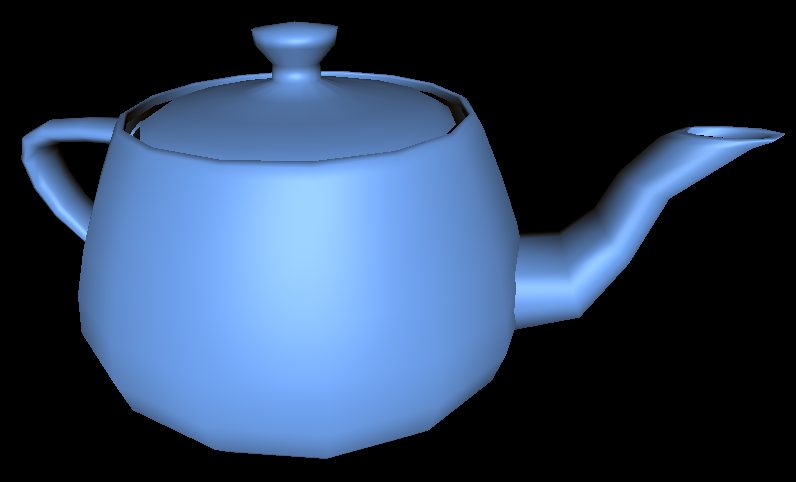
\includegraphics[scale=0.35]{img/cap01/teapotPhong}} \\
  \end{center}
  \caption[Comparación entre los modelos de sombreado de Gouraud y de Phong]{El mismo modelo visto en condiciones geométricas iguales y con el mismo modelo de iluminación pero con dos modelos de sombreado distintos.}
  \label{fig:shadingComparation}
\end{figure}

\subsection{Efectos a partir de mapas para aumentar el realismo de la escena}
\subsubsection{Mapeo de texturas}

Otra técnica de GC que sirve para aumentar realismo a la escena es el mapeo de texturas. La manera mas simple de pensar en el mapeo de texturas es imaginar una calcomanía que se pega a las primitivas geométricas. Por ejemplo podría tratarse de una esfera a la que quisiéramos aplicar un calcomanía de un mapa de la tierra para pensar en un modelo del planeta tierra. El poder representar la superficie de una esfera en el plano ha sido un problema al que se han enfrentado los cartógrafos desde hace muchos años. El mapeo de texturas es el mismo problema pero visto al contrario, queremos poder encontrar una correspondencia entre puntos en una superficie a un plano que representa la textura. De ahí el nombre de mapeo de texturas.

El mapeo de texturas ha avanzado mucho desde los inicio de las GC, por ejemplo ahora es común que las texturas no solo guarden información del color. En su forma más general la textura sirve como una \emph{lookup table}, en la que se guarda alguna propiedad que se asigna a algún píxel de la primitiva por medio de una función. Las propiedades mas comunes que se guardan en la textura son el color, el brillo, los coeficientes de reflexión y las normales. Uno de los ejemplos mas claros es el \emph{bump mapping} que será explicado en la siguiente sección.

El principal reto del mapeo de texturas es definir una función que haga el mapeo. Generalmente un mapa de textura toma las coordenadas $u$ y $v$ en el intervalo $[0, 1]$. Por lo tanto el reto es encontrar una manera de representar la primitiva geométrica como una superficie en coordenadas paramétricas, y luego encontrar un mapeo de los parámetros a coordenadas en el intervalo antes citado.

\begin{figure}[htp]
  \begin{center}
    \subfigure[Primitiva geométrica]{\label{prim}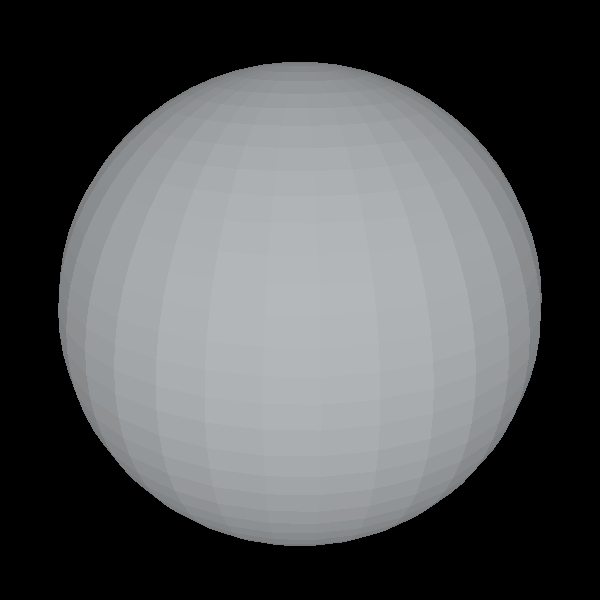
\includegraphics[scale=0.2]{img/cap01/noTexture}}
    \subfigure[Mapa de textura]{\label{textMap}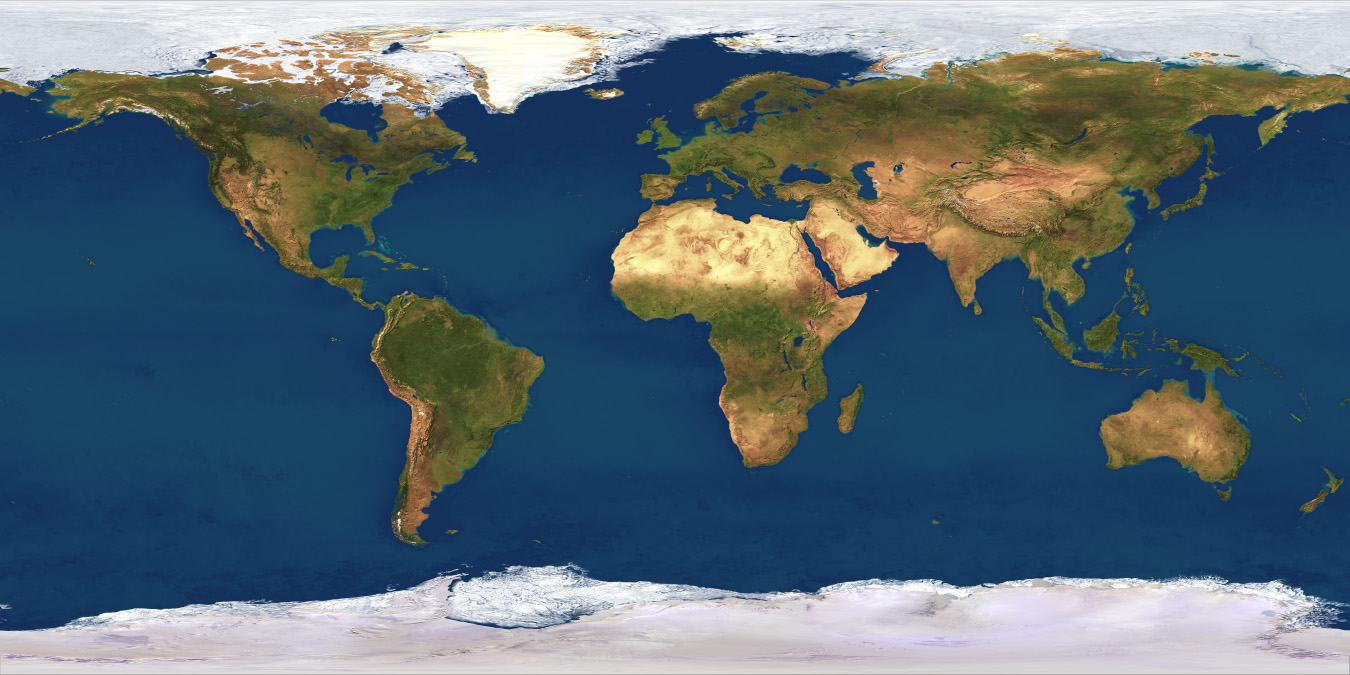
\includegraphics[scale=0.1]{img/cap01/map}}
    \subfigure[Primitiva después de aplicar la textura]{\label{texPrimitive}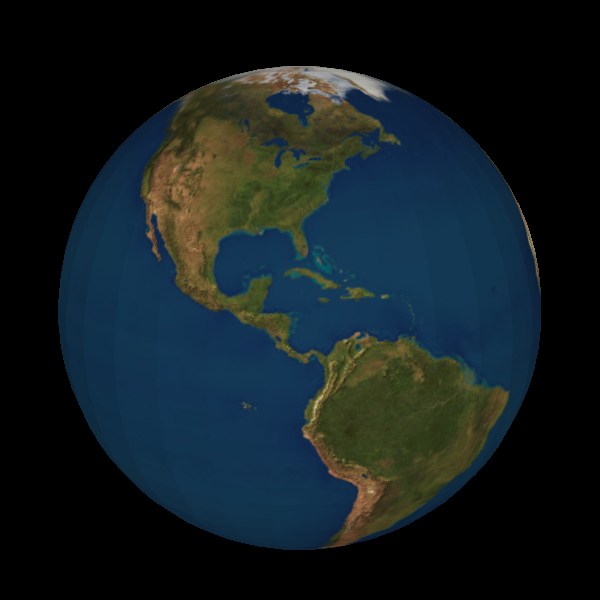
\includegraphics[scale=0.2]{img/cap01/texture}} \\
  \end{center}
  \caption[Mapeo de texturas]{Ejemplo de una primitiva con y sin mapeo de texturas.}
  \label{fig:textureMapping}
\end{figure}

Por ejemplo en la Figura \ref{fig:textureMapping} se hace el mapeo de texturas sobre una esfera. La esfera primero se represento en coordenadas paramétricas de la forma $\textbf{p}(\theta, \phi) = \langle r \sin \theta \cos \phi , r \sin \phi, r \cos \theta \sin \phi \rangle$ en donde $r$ es el radio de la esfera, $\theta \in [0, 2 \pi]$ y $\phi \in [-\frac{\pi}{2}, \frac{\pi}{2}]$ y se ocuparon las siguientes formas para mapear la textura al intervalo $[0, 1]$
\begin{eqnarray}
\nonumber
s & = & \dfrac{\theta}{2 \pi}, \\
t & = & \dfrac{\phi}{\pi} + \dfrac{1}{2}.
\end{eqnarray}

En general, podemos tener problemas cuando no hay una correspondencia uno a uno entre los píxeles de la pantalla y los píxeles del mapa, en este caso pueden pasar dos cosas. Primero que la resolución de los píxeles del mapa sea mucho menor que la resolución de los píxeles de la pantalla, esto se traducirá en que un solo píxel del mapa puede corresponder a varios píxeles de la pantalla. Por lo tanto, veamos que en la pantalla hay regiones grandes de forma aproximadamente rectangular de un sólo color que están correspondiendo a un sólo píxel del mapa.

Segundo, si la resolución del mapa es mucho mayor que la de la pantalla. En un principio esto parecería algo bueno, porque significa que el mapa tiene una resolución mayor que la que necesitamos. Sin embargo, esto también significa que un solo píxel de la pantalla corresponde a varios píxeles en el mapa. Esto implica que sólo algunos de los píxeles del mapa se están usando para producir la imagen final. Lo anterior puede derivar en que aparezcan algunos patrones no deseados en la imagen final. Una primera aproximación para resolver este problema es tratar de utilizar todos los píxeles al momento de hacer el calculo del valor que debería proporcionarnos el mapa. Por ejemplo con una interpolación lineal o con un promedio entre alguna vecindad del píxel seleccionado.

Quizás una de las soluciones mas aceptadas es la propuesta por Williams en \cite{mipmapping}, donde propone la técnica conocida como \emph{mipmapping} que consiste en construir a partir de un mapa original varios mapas de menor resolución hasta llegar a un mapa de un píxel de resolución. Para hacer el mapeo final entonces se calculan: el mapa que está más cerca pero es mayor en resolución y el mapa más cercano pero que es menor en resolución. Luego, en cada mapa se calcula un valor haciendo una interpolación lineal entre los píxeles mas cercanos, lo que produce dos valores. Por último, el valor final se calcula con una interpolación lineal entre la resoluciones de los mapas y la escena. Williams mostró una manera eficiente de hacer este cálculo tanto en tiempo como en memoria. Para guardar los mapas de textura de varias resoluciones solo requiere de 33\% mas espacio que el mapa original. Este algoritmo está actualmente implementado en la mayoría de los procesadores de video (GPU).

Con la llegada de las GPUs programables y de los shaders, se potenció mucho el uso de texturas. Las GPUs permiten romper el pipeline gráfico y poder hacer el mapeo de texturas en varios lugares del pipeline y por lo tanto utilizarlo para varios efectos.

\subsubsection{Mapeo de relieves}

Una forma de utilizar el mapeo de texturas para guardar información que afecta el modelo mas allá de su color es el mapeo de relieves (el término en ingles es \emph{bump mapping} y no existe una buena traducción del término al español, lo mas cercano podría ser mapeo de relieves, o mapeo de bordes). En esta técnica propuesta por Blinn en \cite{bumpmapping}, la idea es guardar un mapa de alturas con cuya información se perturban los vectores normales a la superficie del modelo. Una vez que se hacen los cálculos de iluminación esto da una apariencia rugosa al modelo.

Imaginemos que sobre el modelo se pega una calcomanía con relieve (o bordes) de tal forma que la superficie antes suave del modelo ahora tienen ciertas perturbaciones. Como hacer eso implicaría modificar la posición de los vértices de la superficie y sería muy costoso, se trata de simular el proceso. Con ayuda de la calcomanía, que ahora la llamamos mapa de alturas, podemos saber a dónde habría que mover los vértices del modelo para dar la apariencia deseada. En vez de mover los vértices calculamos el vector normal que tendrían los vértices perturbados y se lo asignamos a los vértices \emph{sin modificar} su posición. En conjunto con el modelo de iluminación podemos dar la apariencia de que lo vértices fueron perturbados sin alterar la geometría del modelo. Un ejemplo puede verse en la Figura \ref{fig:bumpMapping}.

\begin{figure}[htp]
  \begin{center}
    \subfigure[Modelo original]{\label{fig:oriMod}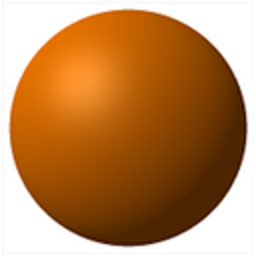
\includegraphics[scale=1.5]{img/cap01/model}}
    \subfigure[Mapa de alturas]{\label{fig:altMap}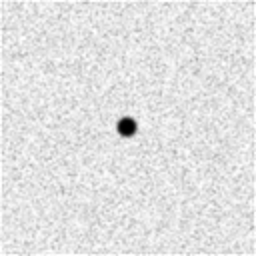
\includegraphics[scale=1.5]{img/cap01/bump}}
    \subfigure[Mapeo de relieves]{\label{fig:bumMap}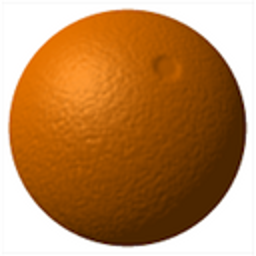
\includegraphics[scale=1.5]{img/cap01/bumpMapping}} \\
  \end{center}
  \caption[Ejemplo de mapeo de relieves]{Ejemplo de mapeo de relieves. Los bordes no están realmente ahí, son artefactos producidos por la iluminación en la escena.}
  \label{fig:bumpMapping}
\end{figure}

Supongamos que tenemos una superficie que puede ser definida de manera paramétrica $\textbf{p}(\mu,\nu)$. Supongamos también que las derivadas parciales $\frac{\partial \textbf{p}}{\partial \mu} = \textbf{p}_\mu$ y $\frac{\partial \textbf{p}}{\partial \nu} = \textbf{p}_\nu$ existen y no son cero en ninguna parte de la superficie.

Podemos encontrar un vector normal unitario a la superficie por medio de la siguiente expresión:
\begin{equation}
\vec{\textbf{n}}(\mu,\nu) = \dfrac{\textbf{p}_\mu \times \textbf{p}_\nu}{\| \textbf{p}_\mu \times \textbf{p}_\nu \|}. 
\label{ec:normalSupParametrica}
\end{equation}

El mapa de bordes puede imaginarse como un mapa de alturas de valores escalares $h(\mu,\nu)$ que representa un desplazamiento de la superficie en dirección de la normal. Ver la Figura \ref{fig:bumpMapDiag} en donde la superficie, representada por la linea negra continua, se desplaza en dirección del vector normal una cierta altura y se aproxima la superficie perturbada (en lineas rojas punteadas).

\begin{figure}[htp]
 \centering
  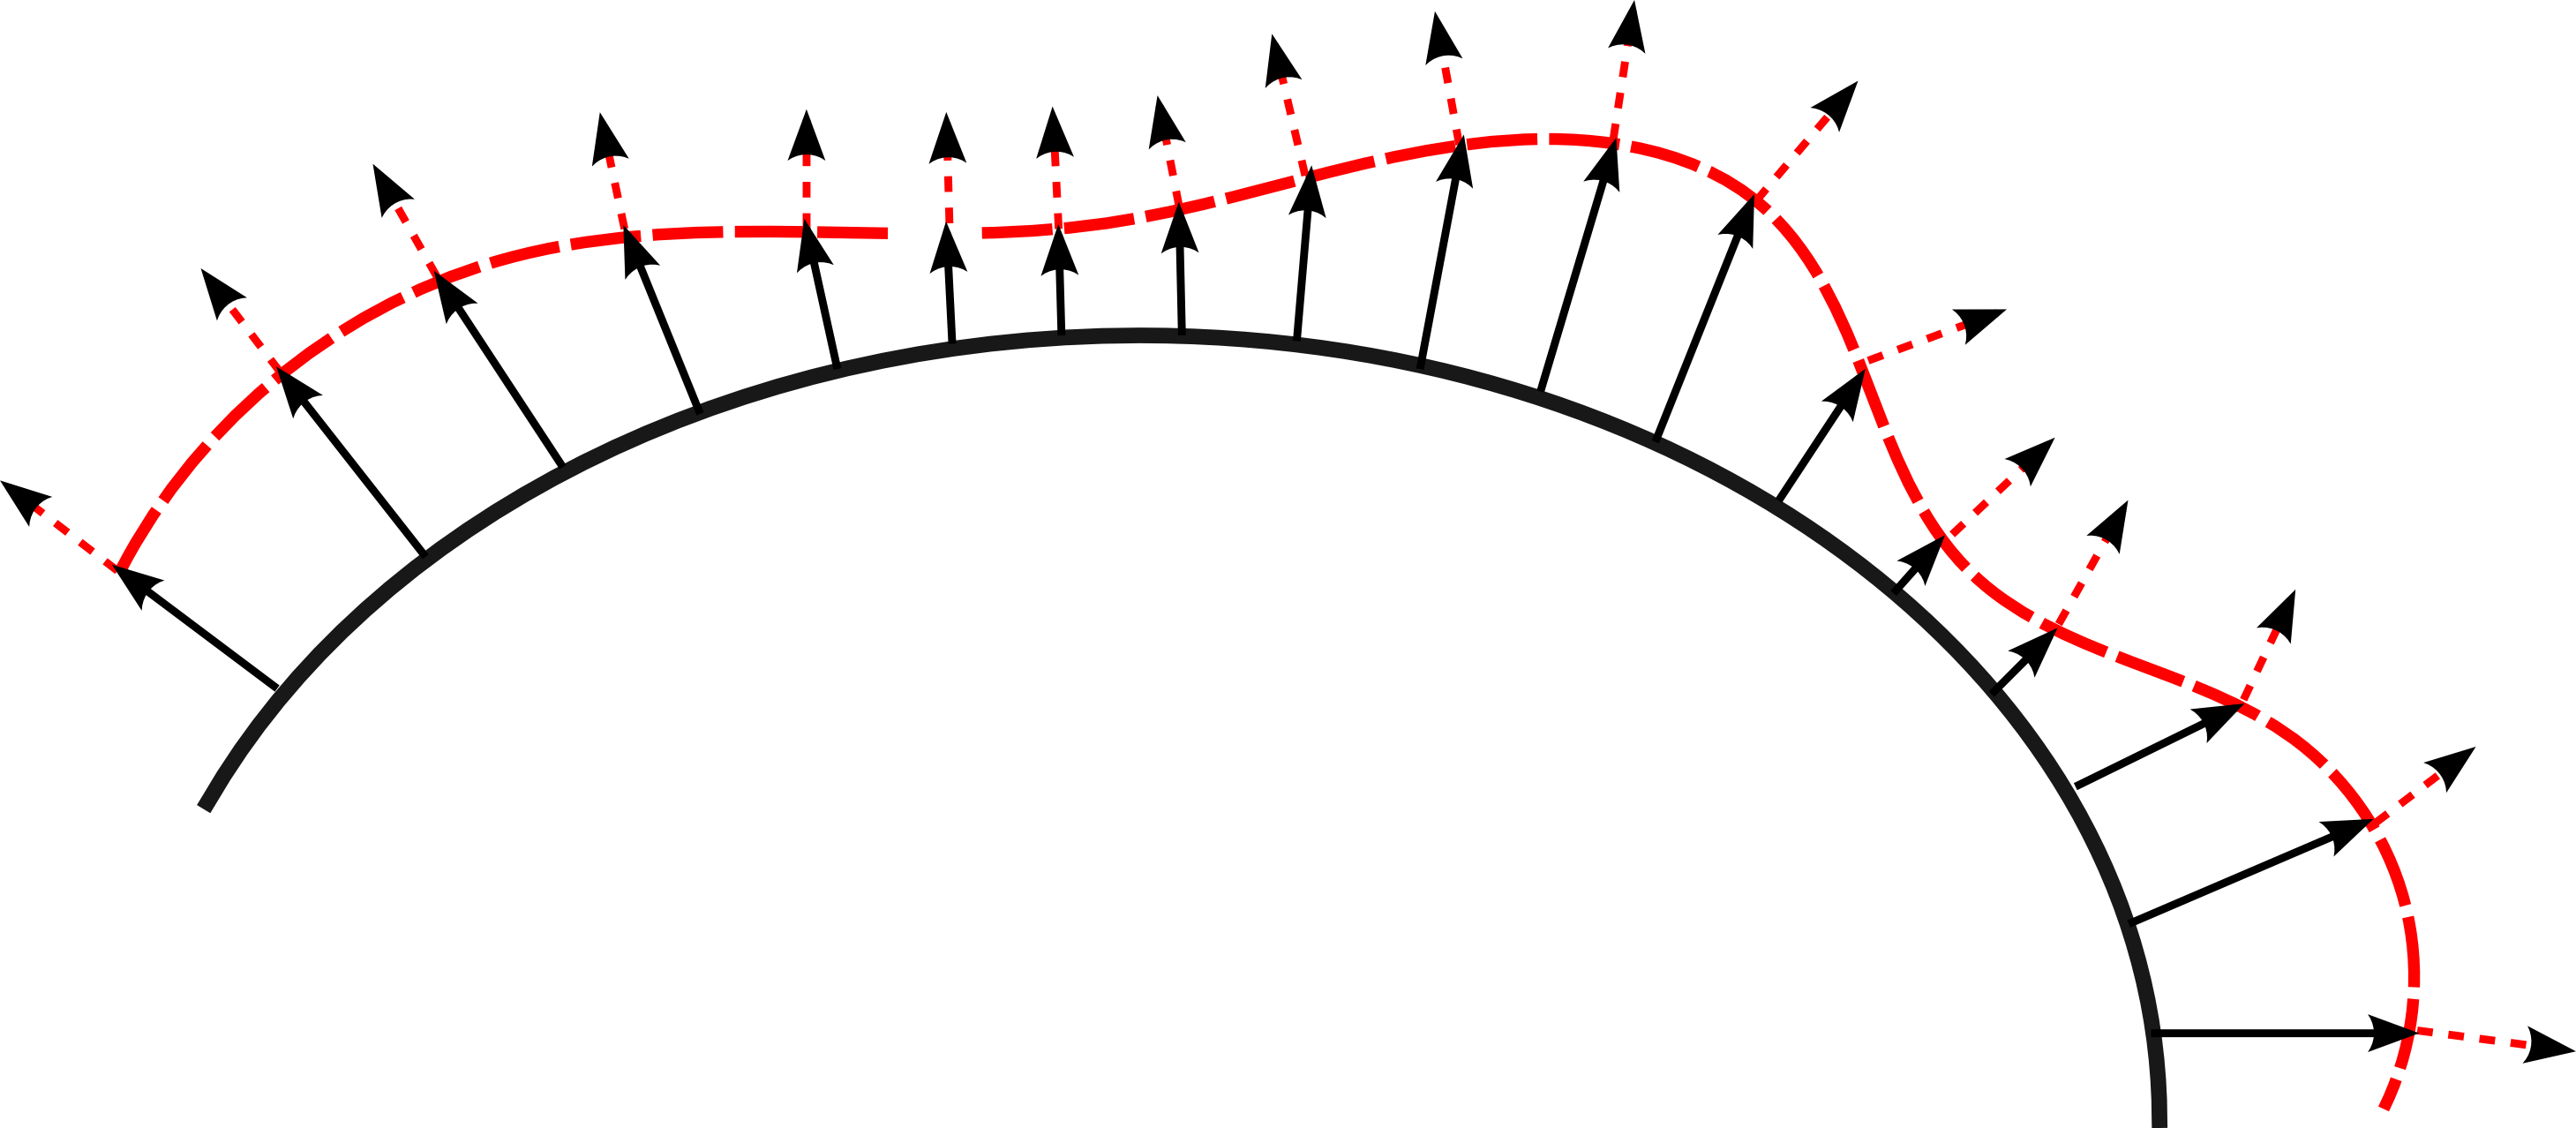
\includegraphics[scale=0.5]{img/cap01/bumpMapDiag}
  \caption[Diagrama geométrico del mapeo de relieves]{La superficie real negra, es perturbada por medio del mapa de alturas $h$, para simular bordes resultando en la superficie roja punteada.}
  \label{fig:bumpMapDiag}
\end{figure}

La fórmula de los puntos en la superficie perturbada $\textbf{p}^{*}$ a partir de la de la superficie real $\textbf{p}$ es
\begin{equation}
\textbf{p}^{*} = \textbf{p} + h \vec{\textbf{n}}.
\label{ec:bumMapPerturbacion}
\end{equation}

En la Figura \ref{fig:bumpMapDiag} las flechas de color negro representan $h \vec{\textbf{n}}$, por lo tanto el mapa de bordes $h$ se traduce en la longitud de estos vectores $\vec{\textbf{n}}$. Por eso decimos que el mapa de bordes es una especie de \emph{mapa de alturas}. Ahora deseamos encontrar las normales a la superficie perturbada, en la Figura \ref{fig:bumpMapDiag} son representadas por las flechas de color rojo y asignar a la superficie real esas normales. Las normales a la superficie perturbada $\textbf{p}^{*}$ pueden calcularse encontrando primero las derivadas parciales
\begin{eqnarray}
\nonumber
\dfrac{\partial \textbf{p}^{*}}{\partial \mu} & = & \frac{\partial \textbf{p}}{\partial \mu} + \frac{\partial h}{\partial \mu} \vec{\textbf{n}} + h \frac{\partial \vec{\textbf{n}}}{\partial \mu}, \\
\dfrac{\partial \textbf{p}^{*}}{\partial \nu} & = & \frac{\partial \textbf{p}}{\partial \nu} + \frac{\partial h}{\partial \nu} \vec{\textbf{n}} + h \frac{\partial \vec{\textbf{n}}}{\partial \nu}.
\end{eqnarray}

En las expresiones anteriores podemos asumir que los últimos términos valen cero. La justificación de esta simplificación es que en general si la superficie original es suave las normales no pueden cambiar mucho a lo largo de ella. Además como sólo permitimos pequeños bordes en la superficie también esperamos que la perturbación $h$ sea pequeña. Sin embargo, como queremos que los bordes se noten no podemos asumir que las derivadas $h_\mu$ y $h_v$ son pequeñas
\begin{eqnarray}
\nonumber
\dfrac{\partial \textbf{p}^{*}}{\partial \mu} & \approx & \frac{\partial \textbf{p}}{\partial \mu} + \frac{\partial h}{\partial \mu} \vec{\textbf{n}}, \\
\dfrac{\partial \textbf{p}^{*}}{\partial \nu} & \approx & \frac{\partial \textbf{p}}{\partial \nu} + \frac{\partial h}{\partial \nu} \vec{\textbf{n}}.
\end{eqnarray}

Ahora el vector normal $\textbf{m}$ que estamos buscando es simplemente el producto cruz de las derivadas parciales
\begin{eqnarray}
\nonumber
\textbf{m}  & \approx & \left( \frac{\partial \textbf{p}}{\partial \mu} + \frac{\partial d}{\partial \mu} \vec{\textbf{n}} \right) \times \left( \frac{\partial \textbf{p}}{\partial v} + \frac{\partial d}{\partial v} \vec{\textbf{n}} \right) \\
& = & \left( \frac{\partial \textbf{p}}{\partial \mu} \times \frac{\partial \textbf{p}}{\partial \nu} \right) + \left( \frac{\partial d}{\partial \mu} \vec{\textbf{n}} \times \frac{\partial \textbf{p}}{\partial \nu} \right) - \left( \frac{\partial d}{\partial \nu} \vec{\textbf{n}} \times \frac{\partial \textbf{p}}{\partial \mu} \right).
\label{ec:normBumpMapping}
\end{eqnarray}

Recordemos que los vectores para iluminación deben ser unitarios, así que en realidad a cada punto de la superficie le asignamos la normal $\vec{\boldsymbol\eta} = \frac{\textbf{m}}{\| \textbf{m} \|}$ este vector es representado por las flechas rojas en la Figura \ref{fig:bumpMapDiag}. También podemos ver de \eqref{ec:normBumpMapping} que $\vec{\boldsymbol\eta}$ no depende explícitamente del mapa de alturas $d$ si no más bien de sus derivadas parciales.

Una aproximación de $h_\mu$ y $h_\nu$ se construye por diferencias finitas en la imagen que representa el mapa. Es también común que en vez de guardar el mapa de alturas se guarden un par de imágenes obtenidas por diferencias finitas sobre la imagen original que directamente representan $h_\mu$ y $h_\nu$.

También se debe señalar que $\vec{\boldsymbol\eta}$ no esta definida en lugares en donde $p_\mu$ o $p_v$ valen cero. Por esta razón se debe de tener cuidado al asignar normales en esas regiones. Una manera de resolver el problema es interpolar linealmente las normales en una cierta vecindad de estos puntos críticos.